% Informe final CBM423. Las cifras provienen de results/ del repositorio (ver results/README.md).
\documentclass[11pt,a4paper]{article}
\usepackage[utf8]{inputenc}
\usepackage[T1]{fontenc}
\IfFileExists{spanish.ldf}{\usepackage[spanish,es-tabla,es-noshorthands]{babel}}{%
  \renewcommand{\figurename}{Figura}\renewcommand{\tablename}{Tabla}%
  \renewcommand{\refname}{Bibliograf\'ia}\renewcommand{\abstractname}{Resumen}\renewcommand{\contentsname}{\'Indice}}
\usepackage{lmodern}
\usepackage[margin=2.4cm]{geometry}
\usepackage{graphicx}
\usepackage{booktabs}
\usepackage{amsmath}
\usepackage{microtype}
\usepackage{caption}
\usepackage{float}
\usepackage[hidelinks]{hyperref}
\usepackage[numbers,sort&compress]{natbib}
\graphicspath{{figures/}}
\captionsetup{font=small,labelfont=bf}
\renewcommand{\arraystretch}{1.1}
\setlength{\parskip}{3pt}
\emergencystretch=2em

\title{Segmentación de masas mamarias en mamografía (CBIS-DDSM):\\
U-Net, morfología aprendible y SegFormer, y los límites de derivar la forma BI-RADS desde la máscara}
\author{Anielly Yañez Felicio\\
\small Ingeniería Civil Biomédica, Universidad de Valparaíso\\
\small CBM423 -- Procesamiento Digital de Imágenes Médicas}
\date{9 de diciembre de 2026}

\begin{document}
\maketitle

\begin{abstract}
Se segmentan masas mamarias en recortes de región de interés (ROI) del conjunto CBIS-DDSM con una U-Net y se la compara con dos referencias (Otsu con morfología y un control que solo usa la posición de la lesión), con una variante que incorpora capas morfológicas aprendibles, con un posprocesamiento morfológico fijo y con SegFormer-B0, un transformer pequeño. Con el protocolo final (partición por paciente, selección solo en validación, tres semillas, test oficial de 378 masas), la U-Net alcanza Dice $0.762 \pm 0.009$ frente a $0.32$--$0.35$ de las referencias. La morfología aprendible dentro de la red no mejora ($0.762 \pm 0.001$); el posprocesamiento fijo reduce la distancia de Hausdorff 95 de 25.6 a 18.3 px, pero su efecto sobre el Dice no se confirma en test. SegFormer-B0 es el mejor modelo ($0.792 \pm 0.003$); la ventaja se atribuye sobre todo a la arquitectura (el aporte del preentrenamiento no es concluyente) y no se explica por una menor confusión con otras estructuras densas. El Dice depende de la dificultad de la imagen (sutileza, densidad mamaria) y no del tipo de lesión. Por último, la forma y el margen BI-RADS no se recuperan desde la geometría de las máscaras (AUC $\approx 0.5$ incluso con las máscaras anotadas), aunque las etiquetas del radiólogo sí predicen la patología (AUC $\approx 0.78$): el límite está en las máscaras del conjunto, no en la red.
\end{abstract}

%==================================================================
\section{Introducción y objetivos}
La segmentación automática de masas es un paso básico de los sistemas de apoyo al diagnóstico en mamografía. La forma de la masa (redonda, ovalada, lobulada o irregular) y su margen son descriptores del léxico BI-RADS asociados al riesgo de malignidad. La edición BI-RADS v2025 reintroduce ``lobulada'' como forma y elimina ``microlobulado'' como margen \citep{acr2025birads}; CBIS-DDSM \citep{lee2017cbisddsm} ya incluye la forma lobulada en su campo \texttt{mass shape}. Los trabajos previos con U-Net y variantes sobre CBIS-DDSM e INbreast reportan Dice muy variables, aproximadamente de 0.4 a 0.95 según el protocolo (ROI o mamografía completa, subconjunto, preprocesamiento) \citep{abdelhafiz2020,baccouche2021connected}, por lo que una comparación directa con la literatura exige cautela.

\paragraph{Objetivo general.} Entrenar modelos que segmenten masas mamarias en recortes ROI de CBIS-DDSM, compararlos con enfoques tradicionales y analizar críticamente dónde fallan. Los objetivos específicos son:
\begin{enumerate}
\item[\textbf{O1.}] Segmentar con una U-Net y compararla con Otsu más morfología y con un ``prior centrado'' (un círculo fijo en el centro, que mide cuánto Dice se explica solo por la posición).
\item[\textbf{O2.}] Incorporar morfología en capas convolucionales y comparar con otra familia de modelos distinta de la U-Net.
\item[\textbf{O3.}] Analizar el error según sutileza, densidad, patología, forma y margen BI-RADS anotados, y los modos de fallo.
\item[\textbf{O4.}] Evaluar si la forma (y el margen) BI-RADS pueden derivarse de la máscara mediante descriptores geométricos y un clasificador interpretable.
\end{enumerate}

\subsection{Cambios respecto de la entrega parcial}
La Tabla~\ref{tab:cambios} resume lo que cambió respecto del informe de avance del 15 de octubre, con su motivo.

\begin{table}[H]
\centering\small
\caption{Cambios entre la entrega parcial y la final.}
\label{tab:cambios}
\begin{tabular}{p{3.3cm}p{5.4cm}p{6cm}}
\toprule
Aspecto & Entrega parcial & Entrega final \\
\midrule
Cifra principal de la U-Net & Dice test 0.771 (una corrida, semilla 42) & $0.762 \pm 0.009$ (3 semillas); una nueva ejecución de la semilla 42 dio 0.769 (no determinismo de cuDNN). \\
Segunda arquitectura & Attention U-Net o U-Net++ (plan) & Sustituida por dos propuestas de la retroalimentación del profesor: capas morfológicas aprendibles (Morph-UNet) y otra familia, SegFormer-B0. La Attention U-Net no se realizó. \\
Objetivo 3 (forma) & Reformulado: documentar la limitación y estratificar el Dice por forma y margen (pendiente) & Realizado: análisis estratificado, margen BI-RADS desde la geometría (también negativo) y análisis de fallos. \\
Fallos de localización & 13 de 378 recortes con Dice $<0.1$; 10 en el tercil de mayor desplazamiento & 16 de 378 en la semilla 42 (13.3 de media entre semillas); 9 de 16 en el tercil alto, y el desplazamiento los explica solo en parte. \\
Métricas de borde & Pendiente & Hausdorff 95 (HD95) incorporado. \\
Estadística & Una sola corrida & 3 semillas, validación cruzada de 5 particiones por paciente, IC por bootstrap y Wilcoxon pareado. \\
\bottomrule
\end{tabular}
\end{table}

%==================================================================
\section{Datos}
Se usa CBIS-DDSM \citep{lee2017cbisddsm}, versión curada de DDSM \citep{heath2001ddsm}, en su copia de Kaggle (carpetas \texttt{csv/} y \texttt{jpeg/}); los datos no forman parte del repositorio. Se trabaja con el subconjunto de masas y sus divisiones oficiales: 1318 lesiones de entrenamiento (691 pacientes) y 378 de test (201 pacientes). Las 1318 se dividen \emph{por paciente} en 1061 (entrenamiento) y 257 (validación), de modo que ningún paciente queda en dos conjuntos. El test oficial se reserva para informar resultados y no se usa para elegir nada.

\paragraph{Hallazgos de datos que condicionaron el diseño.}
(i)~Las rutas del CSV no coinciden con las carpetas de la copia de Kaggle, y recorte y máscara comparten carpeta sin etiqueta; se distinguen porque la máscara es casi binaria.
(ii)~La máscara está en las coordenadas de la \emph{mamografía completa}, no del recorte oficial; por eso se generan recortes propios.
(iii)~Con un primer recorte centrado en la lesión, un círculo fijo lograba Dice 0.857, es decir, la posición quedaba ``regalada''; se corrigió con contexto $3\times$ y desplazamiento aleatorio (Sección~\ref{sec:ablaciones}).
(iv)~La alineación se verificó: cada recorte coincide con su fila del CSV (1696 de 1696) y el interior de la máscara es más brillante que el exterior en el 98.1\,\% de los casos.

\paragraph{Etiquetas de forma y margen.} 1100 de las 1318 lesiones de entrenamiento (324 de 378 en test) tienen una de las 4 formas básicas (irregular 351, ovalada 321, lobulada 305, redonda 123 en entrenamiento); las formas combinadas y otras categorías (ganglio linfático, distorsión arquitectural, asimetrías) se excluyen del análisis de forma, pero no del de segmentación.

\begin{figure}[H]
  \centering
  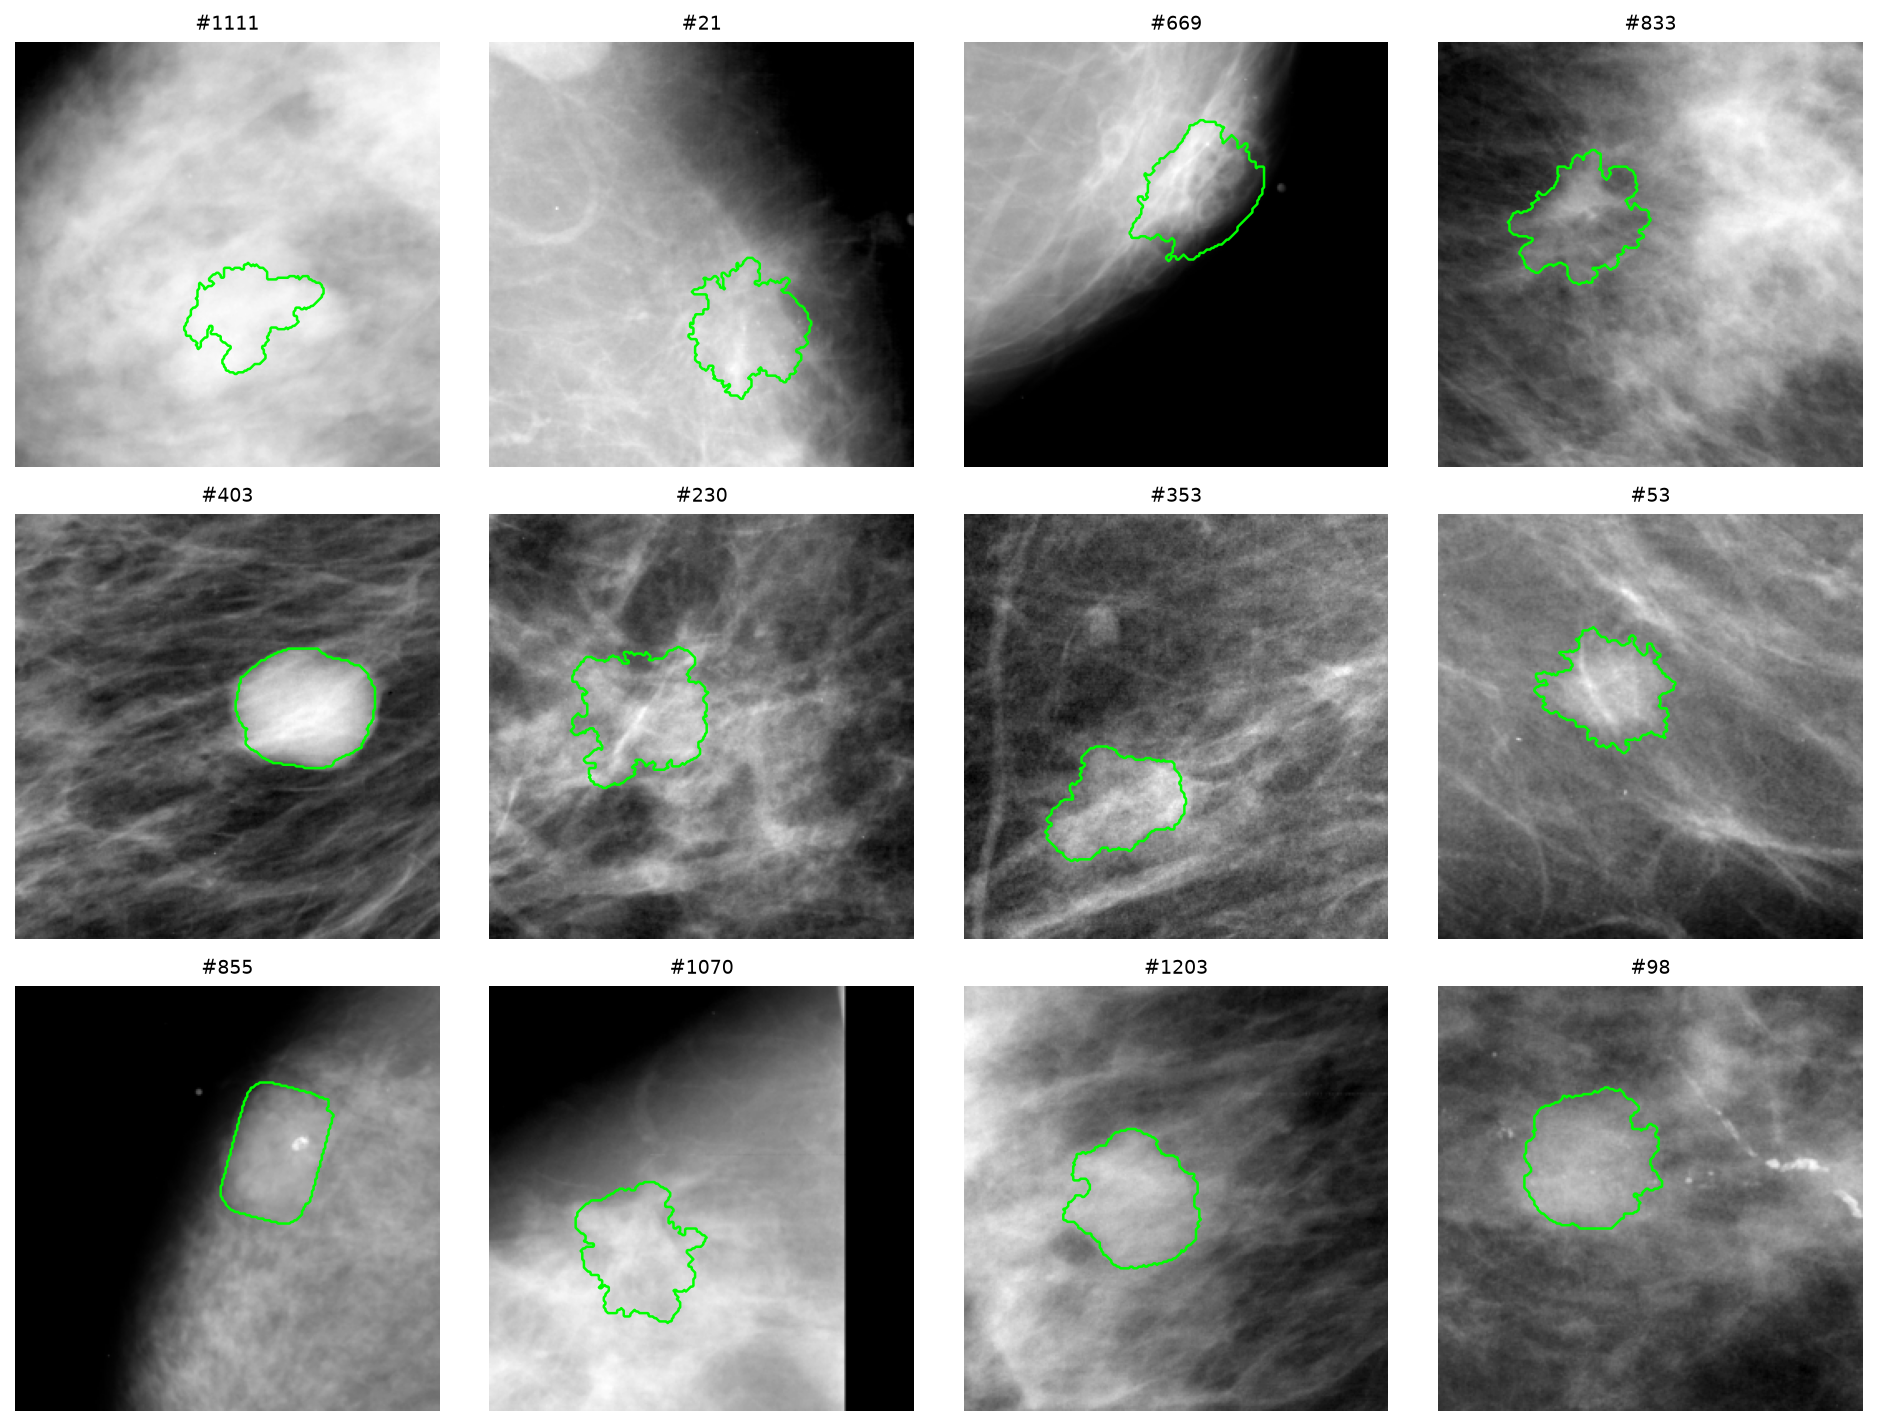
\includegraphics[width=\linewidth]{muestras_recortes.png}
  \caption{Recortes ROI propios con el contorno anotado.}
  \label{fig:recortes}
\end{figure}

%==================================================================
\section{Métodos}
\subsection{Recortes ROI con desplazamiento aleatorio}
Para cada lesión se binariza la máscara y se obtiene su caja; el lado del recorte es $L=\max(3\max(b_h,b_w),\,96)$ px, de modo que la lesión ocupa cerca de un tercio del lado. El centro se desplaza al azar hasta $\pm 20\,\%$ de $L$ por eje (semilla fija por fila). Se recorta un cuadrado de la mamografía y de la máscara, se reescala a $256\times256$ y se normaliza la imagen por percentiles 1--99. La lesión ocupa en promedio cerca del 6\,\% del recorte. No se usan los recortes oficiales porque no están registrados con la máscara.

\subsection{Modelos de segmentación}
\paragraph{Referencias.} \emph{Prior centrado:} un círculo en el centro con el área media de las lesiones de entrenamiento. \emph{Clásico:} suavizado gaussiano ($\sigma=2$), umbral de Otsu \citep{otsu1979} calculado en una ventana central, apertura y cierre con disco de radio 3, relleno de huecos y componente conexa más cercana al centro.

\paragraph{U-Net.} Arquitectura de \citet{ronneberger2015unet} con 4 niveles, 16 filtros base y 1.94 M de parámetros (Conv--BatchNorm--ReLU y conexiones de salto). Pérdida BCE más Dice \citep{milletari2016vnet}, AdamW \citep{loshchilov2019adamw} (lr $10^{-3}$), ReduceLROnPlateau sobre el Dice de validación, lote 8, hasta 40 épocas con detención temprana (paciencia 10), recorte de gradiente 1.0 y aumento de datos en GPU (volteos, rotación, escala, traslación, contraste y brillo). La precisión mixta se desactiva porque produce pérdida NaN en la GPU disponible (GTX 1650, 4 GB). Implementada en PyTorch \citep{paszke2019pytorch}; unos 16 s por época.

\paragraph{Morph-UNet (capas morfológicas aprendibles).} Siguiendo la recomendación del profesor, se agrega a la U-Net un bloque con \emph{p-convoluciones} (media contraarmónica; \citealp{masci2013morph,kirszenberg2021pconv}). Dada una imagen positiva $x$ y un elemento estructurante $w$, la capa calcula $y=\operatorname{conv}(x^{p+1},w)/\operatorname{conv}(x^{p},w)$, que se aproxima a una dilatación para $p\gg 0$ y a una erosión para $p\ll 0$; $p$ y $w$ se aprenden. Se implementa de forma numéricamente estable como $\operatorname{softmax}(p\log x+\log w)$ sobre ventanas de $5\times5$, y las pruebas la comparan con \texttt{scipy.ndimage} para $|p|$ grande. El bloque reduce a 4 canales con una convolución $1\times1$, aplica en paralelo una apertura (erosión y dilatación) y un cierre (dilatación y erosión), expande de nuevo y suma con conexión residual. Agrega solo 628 parámetros, pero cada época tarda 59 s (3.7 veces más) y necesita \emph{gradient checkpointing} para caber en 4 GB. Se probaron dos ubicaciones, antes de la cabeza $1\times1$ y en la conexión de salto de máxima resolución, y se eligió esta última con la validación (semilla 42).

\paragraph{Posprocesamiento morfológico fijo.} Apertura y cierre con un disco de radio $r$ y conservación de la componente conexa mayor, aplicado a las predicciones de la U-Net. El radio se eligió solo en validación ($r=6$), aunque, como se verá, es prácticamente equivalente a $r=0$.

\paragraph{SegFormer-B0.} Transformer pequeño con atención global y decodificador MLP \citep{xie2021segformer}: codificador MiT-b0 preentrenado en ImageNet-1k (\texttt{nvidia/mit-b0}, vía \texttt{transformers}), decodificador inicializado al azar, entrada de 1 canal replicada a 3 y salida de 1 canal a $64\times64$ escalada a $256\times256$ por interpolación bilineal. Tiene 3.71 M de parámetros, 29--34 s por época y 1.1 GB de GPU. Misma pérdida, optimizador, lote, detención temprana y aumento que la U-Net; el lr se eligió solo en validación entre $10^{-4}$ y $3\times10^{-4}$ (semilla 42), con $3\times10^{-4}$ como ganador. Como control se entrena también sin preentrenamiento (pesos aleatorios).

\subsection{Forma y margen desde la geometría}
De cada máscara se calculan 8 descriptores (circularidad, solidez, excentricidad, razón de ejes, número de concavidades, rugosidad, variación radial y número de lóbulos), con suavizado opcional del contorno ($\sigma\in\{0,2,4\}$ px). Un árbol de decisión de profundidad 3, una regresión logística y un \emph{random forest} \citep{pedregosa2011sklearn,vanderwalt2014skimage} asignan una de las 4 formas. Para el margen se agrupa en M1 (circunscrito frente a no circunscrito) y M2 (espiculado frente al resto), excluyendo los márgenes ``obscured'' solos, las mezclas con ``circumscribed'' y los casos sin dato. En todos los casos el ajuste es en entrenamiento, la elección del suavizado y el clasificador en validación, y el test se evalúa una sola vez con la combinación elegida. Se añaden controles que predicen la patología desde los descriptores, desde la etiqueta de forma del radiólogo y desde su combinación.

\subsection{Métricas y evaluación estadística}
Dice, IoU, precisión y sensibilidad por recorte; y la distancia de Hausdorff 95 (HD95), el percentil 95 de las distancias entre contornos, en píxeles del recorte de $256\times256$ (las predicciones vacías no tienen HD95 y se cuentan aparte). Para la forma: exactitud, exactitud balanceada, F1 macro y AUC. Toda comparación o selección usa validación o validación cruzada; el test solo informa. Se reportan la media $\pm$ desviación estándar de 3 semillas de entrenamiento, una validación cruzada de 5 particiones agrupadas por paciente en el entrenamiento oficial, intervalos de confianza de 95\,\% por bootstrap (1000 remuestreos, por recorte y por paciente), prueba de Wilcoxon pareada para diferencias entre modelos, Kruskal-Wallis con corrección de Holm para subgrupos y McNemar exacto para comparar fallos. El código, las configuraciones y 47 pruebas automáticas están en el repositorio (Anexo~\ref{sec:repro}).

%==================================================================
\section{Resultados}
\subsection{Segmentación principal}
La Tabla~\ref{tab:principal} reúne todos los métodos con el mismo protocolo. La U-Net duplica el Dice de las dos referencias: en test $0.762 \pm 0.009$ frente a $0.324$ (clásico) y $0.352$ (prior). El método clásico sobresegmenta (sensibilidad $0.87$, precisión $0.24$): Otsu incluye tejido denso vecino. La diferencia U-Net $-$ clásico es $+0.445$ [IC 95\,\% $0.420$, $0.469$], Wilcoxon $p\approx 5\times10^{-60}$, y la U-Net es mejor en el 94\,\% de los recortes. La validación cruzada por paciente da $0.771 \pm 0.014$ (prior $0.348 \pm 0.021$), y el test ($0.762$) cae dentro de ese rango: no hay indicio de sobreajuste a la partición de validación. En la semilla 42, el IC 95\,\% de la U-Net en test es $0.769$ [$0.746$, $0.791$] por recorte y [$0.746$, $0.795$] por paciente.

\begin{table}[H]
\centering\footnotesize\setlength{\tabcolsep}{3.5pt}
\caption{Segmentación (media $\pm$ DE de 3 semillas para los modelos entrenados; las referencias son deterministas). HD95 medio en px; ``vacías'' es el número medio de predicciones vacías por semilla (test).}
\label{tab:principal}
\begin{tabular}{lccccc}
\toprule
Método & Dice val & Dice test & IoU test & HD95 test & Vacías \\
\midrule
Prior centrado & 0.344 & 0.352 & 0.236 & -- & -- \\
Clásico (Otsu + morfología) & 0.348 & 0.324 & 0.220 & -- & -- \\
U-Net & $0.777 \pm 0.003$ & $0.762 \pm 0.009$ & $0.652$ & 25.6 & 2.3 \\
U-Net + posprocesamiento fijo ($r=6$) & $0.791 \pm 0.006$ & $0.767 \pm 0.007$ & $0.662$ & 18.3 & 7.3 \\
Morph-UNet (bloque en el salto) & $0.777 \pm 0.000$ & $0.762 \pm 0.001$ & $0.650$ & 26.6 & 1.3 \\
SegFormer-B0 sin preentrenar & $0.801 \pm 0.005$ & $0.783 \pm 0.001$ & $0.674$ & 19.0 & 0 \\
\textbf{SegFormer-B0 (preentrenado)} & $\mathbf{0.810 \pm 0.001}$ & $\mathbf{0.792 \pm 0.003}$ & $\mathbf{0.683}$ & 17.4 & 0 \\
SegFormer-B0 + posprocesamiento ($r=6$) & $0.810 \pm 0.003$ & $0.793 \pm 0.003$ & $0.686$ & 16.9 & 0 \\
\bottomrule
\end{tabular}
\end{table}

\begin{figure}[H]
  \centering
  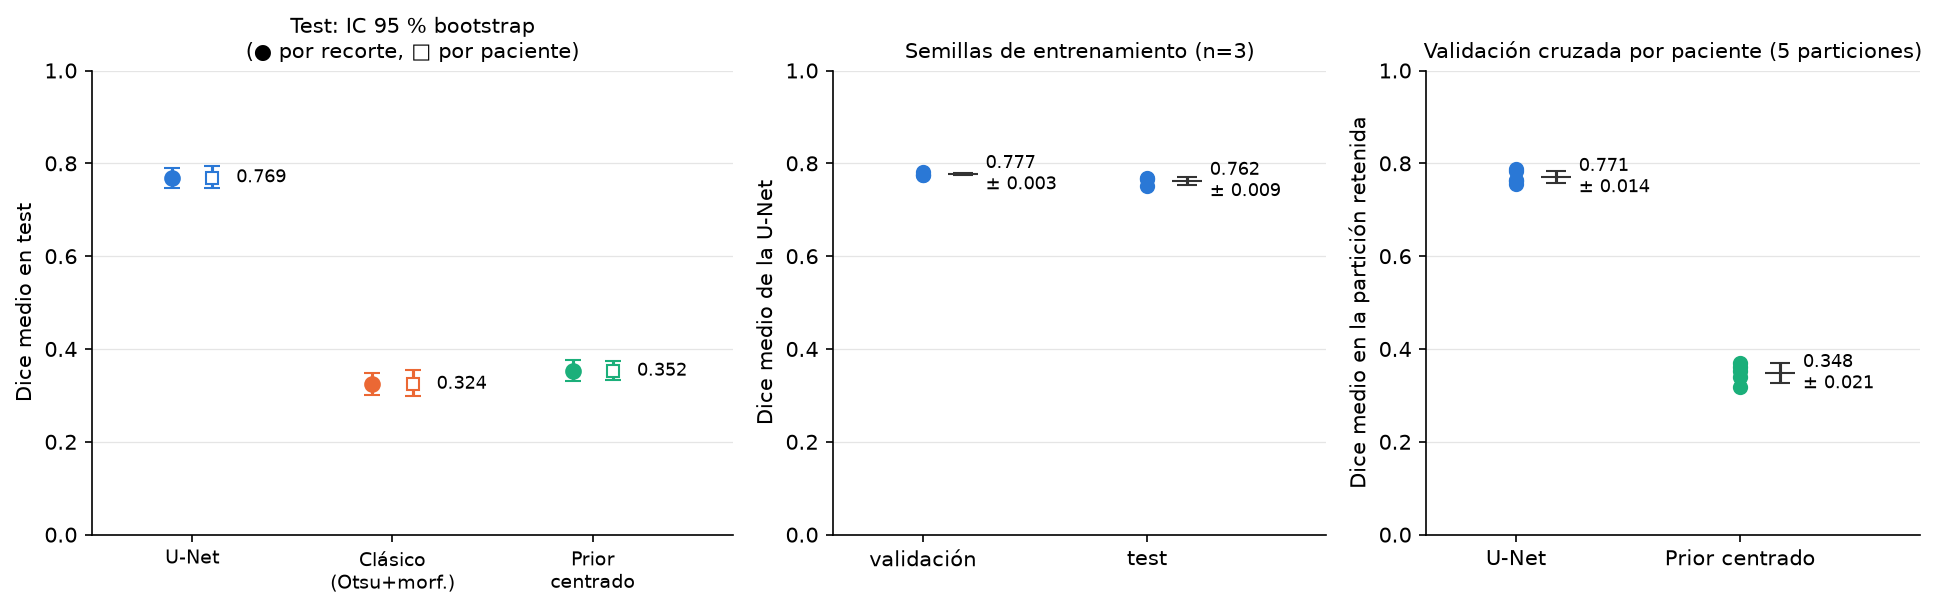
\includegraphics[width=0.95\linewidth]{variabilidad_incertidumbre.png}
  \caption{Intervalos de confianza al 95\,\% en test, dispersión entre semillas y entre particiones de la validación cruzada.}
  \label{fig:variabilidad}
\end{figure}

\begin{figure}[H]
  \centering
  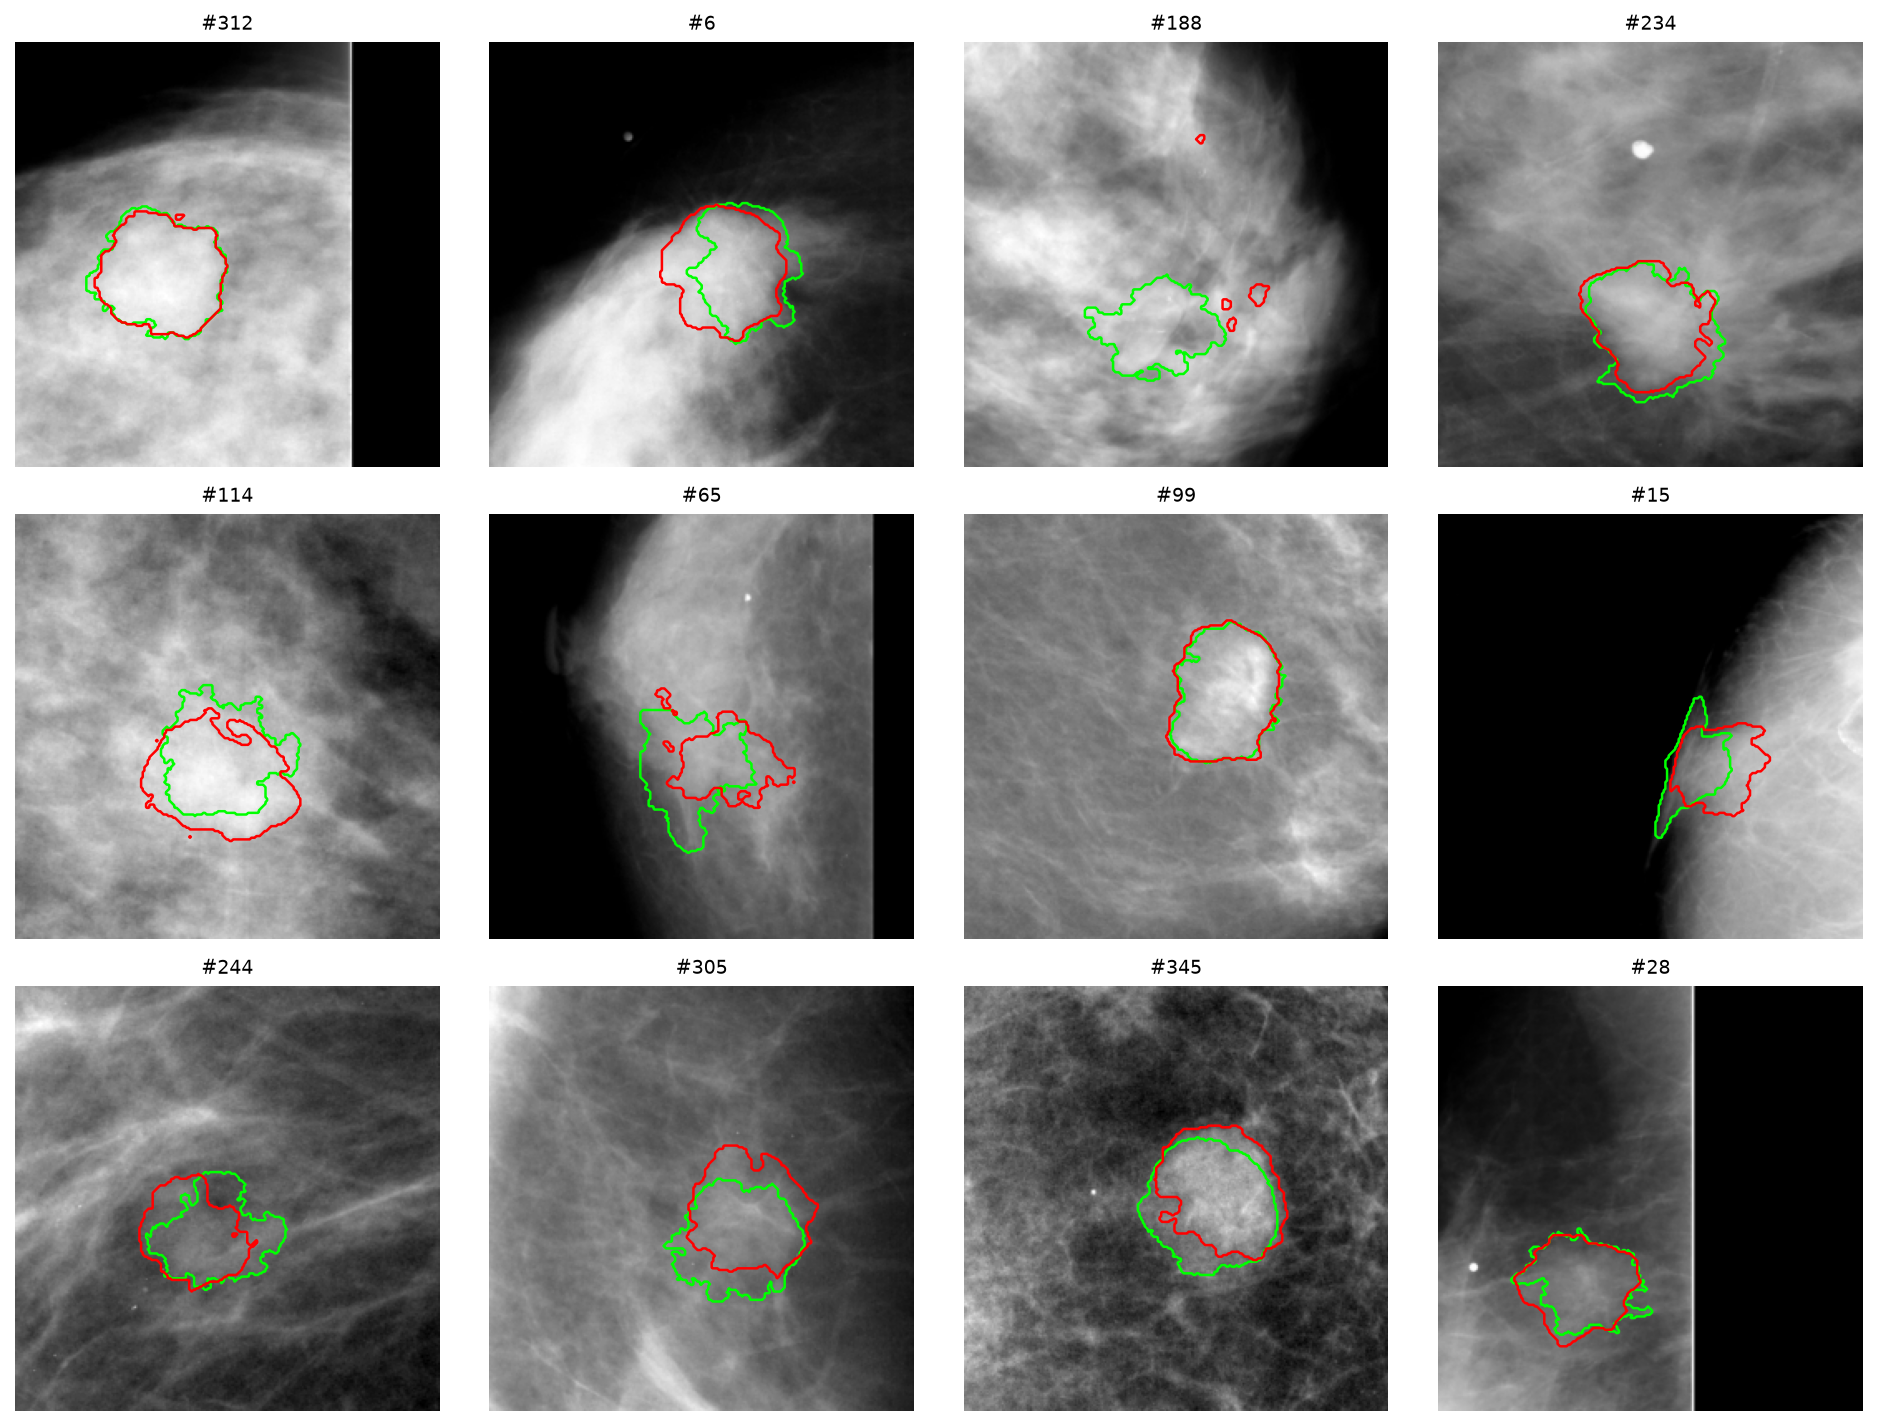
\includegraphics[width=0.95\linewidth]{predicciones_test.png}
  \caption{Predicciones de la U-Net en test: contorno anotado y predicho.}
  \label{fig:predicciones}
\end{figure}

\subsection{Ablaciones y el atajo de posición}\label{sec:ablaciones}
La Tabla~\ref{tab:ablaciones} (solo validación, semilla 42) muestra el hallazgo más importante del diseño de los datos: \emph{sin desplazamiento aleatorio} (jitter 0), un círculo fijo en el centro logra Dice 0.857 y supera a la U-Net (0.839); con jitter, el prior cae a 0.16 mientras la U-Net baja solo a 0.75. Con jitter 0 el Dice mide sobre todo la posición de la lesión en el recorte y no la calidad de la segmentación, por lo que se mantuvo jitter 0.2 aunque dé un Dice menor. Un contexto menor sube el Dice, pero también el del prior: la tarea se hace más fácil, no mejor resuelta; contexto y jitter se informan de forma descriptiva y no se usaron para elegir. Duplicar los canales (con 2.3 veces más tiempo por época) o usar solo Dice como pérdida no mejoran ($-0.014$ cada uno), diferencias del orden del ruido entre semillas, por lo que se mantuvo la configuración más simple.

\begin{table}[H]
\centering\small
\caption{Ablaciones en validación (semilla 42). La referencia es contexto 3, jitter 0.2, base 16, BCE + Dice.}
\label{tab:ablaciones}
\begin{tabular}{lccl}
\toprule
Variante & Dice U-Net & Dice prior & Lectura \\
\midrule
Referencia & 0.781 & 0.345 & -- \\
Contexto 2 / 4 & 0.802 / 0.762 & 0.531 / 0.207 & tarea más fácil / más difícil \\
Jitter 0 / 0.1 / 0.3 & 0.839 / 0.825 / 0.753 & \textbf{0.857} / 0.631 / 0.161 & sin jitter, el prior supera a la U-Net \\
Base 32 & 0.767 & 0.345 & no mejora; 2.3 veces más lento \\
Solo Dice & 0.767 & 0.345 & no mejora \\
\bottomrule
\end{tabular}
\end{table}

\begin{figure}[H]
  \centering
  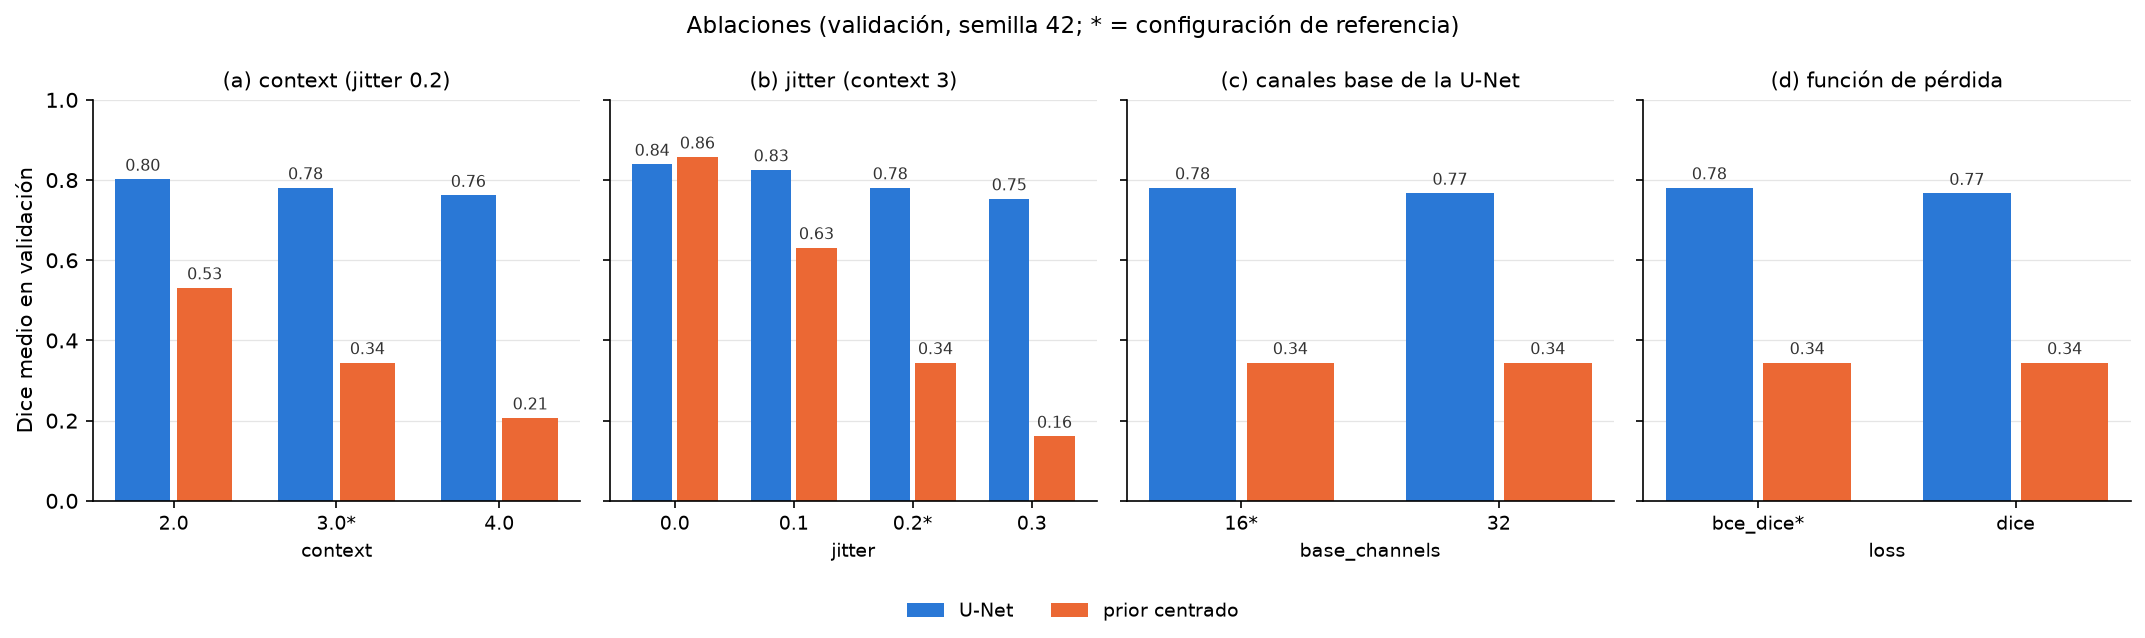
\includegraphics[width=0.95\linewidth]{ablaciones.png}
  \caption{Ablaciones en validación. Sin desplazamiento (jitter 0) el prior centrado supera a la U-Net.}
  \label{fig:ablaciones}
\end{figure}

\subsection{Morfología en la red y posprocesamiento}
\paragraph{La morfología aprendible no mejora.} La Morph-UNet empata con la U-Net en validación y en test (diferencia de Dice $-0.001$ [$-0.006$, $0.005$] en test, Wilcoxon $p=0.65$; HD95 $+0.8$ px, sin significación), con 3.7 veces más tiempo por época. Los valores de $p$ aprendidos casi no se movieron de su inicio ($\pm5$, rango 4.2--5.5), de modo que las capas siguen siendo erosiones y dilataciones suaves, y con la conexión residual la red puede ignorar el bloque. La causa de fondo es otra: los errores dominantes de la U-Net son de localización (segmenta otra estructura densa; Sección~\ref{sec:fallos}), y una operación local de $5\times5$ no puede corregirlos. Cabe la cautela de que la semilla 43 alcanzó su mejor resultado en la última época (40), así que con más épocas podría mejorar algo.

\paragraph{El posprocesamiento fijo mejora el contorno.} El HD95 baja de 26.6 a 16.6 px en validación y de 25.6 a 18.3 px en test (significativo en ambos), porque el 32--34\,\% de las predicciones de la U-Net tiene más de una componente conexa y el filtro elimina las manchas falsas. El Dice sube $+0.014$ en validación (significativo), pero en test solo $+0.004$ con un intervalo que toca el cero ([$-0.000$, $0.009$], $p=0.15$).

\paragraph{Sensibilidad al radio.} Se analizó a posteriori el efecto del radio (Tabla~\ref{tab:radio}; análisis descriptivo, no usado para elegir). En validación todos los radios empatan (0.790--0.791, con DE entre semillas de 0.006), y casi toda la ganancia viene de \emph{quedarse con la componente conexa mayor} ($r=0$ ya da 0.791): la apertura y el cierre no aportan nada medible. En test, un radio mayor deja más predicciones vacías (de 2.3 a 7.3 con $r=6$). La principal causa de recortes que el filtro lleva a Dice $<0.1$ cuando la U-Net no fallaba es que la componente mayor es la equivocada (la U-Net segmenta la lesión y además otra estructura densa más grande; 9 casos en validación y 19 en test, sumando las 3 semillas), mientras que la apertura deja la máscara vacía solo en 1 y 2 casos. La conclusión es que el efecto morfológico útil es la selección de componente, y que la elección $r=6$ (hecha en validación) es indistinguible de $r=0$, que es más simple.

\begin{table}[H]
\centering\small
\caption{Sensibilidad del posprocesamiento al radio $r$ (media de 3 semillas; análisis posterior).}
\label{tab:radio}
\begin{tabular}{lcccccc}
\toprule
 & Dice val & HD95 med.\ val & Dice test & HD95 med.\ test & Vacías test & Dice $<0.1$ test \\
\midrule
Sin posproc. & 0.777 & 13.7 & 0.762 & 15.4 & 2.3 & 13.3 \\
$r=0$ & 0.791 & 11.7 & 0.769 & 12.9 & 2.3 & 20.0 \\
$r=6$ (elegido) & 0.791 & 12.4 & 0.767 & 13.1 & 7.3 & 21.3 \\
$r=8$ & 0.790 & 12.4 & 0.764 & 13.1 & 9.3 & 22.0 \\
\bottomrule
\end{tabular}
\end{table}

\begin{figure}[H]
  \centering
  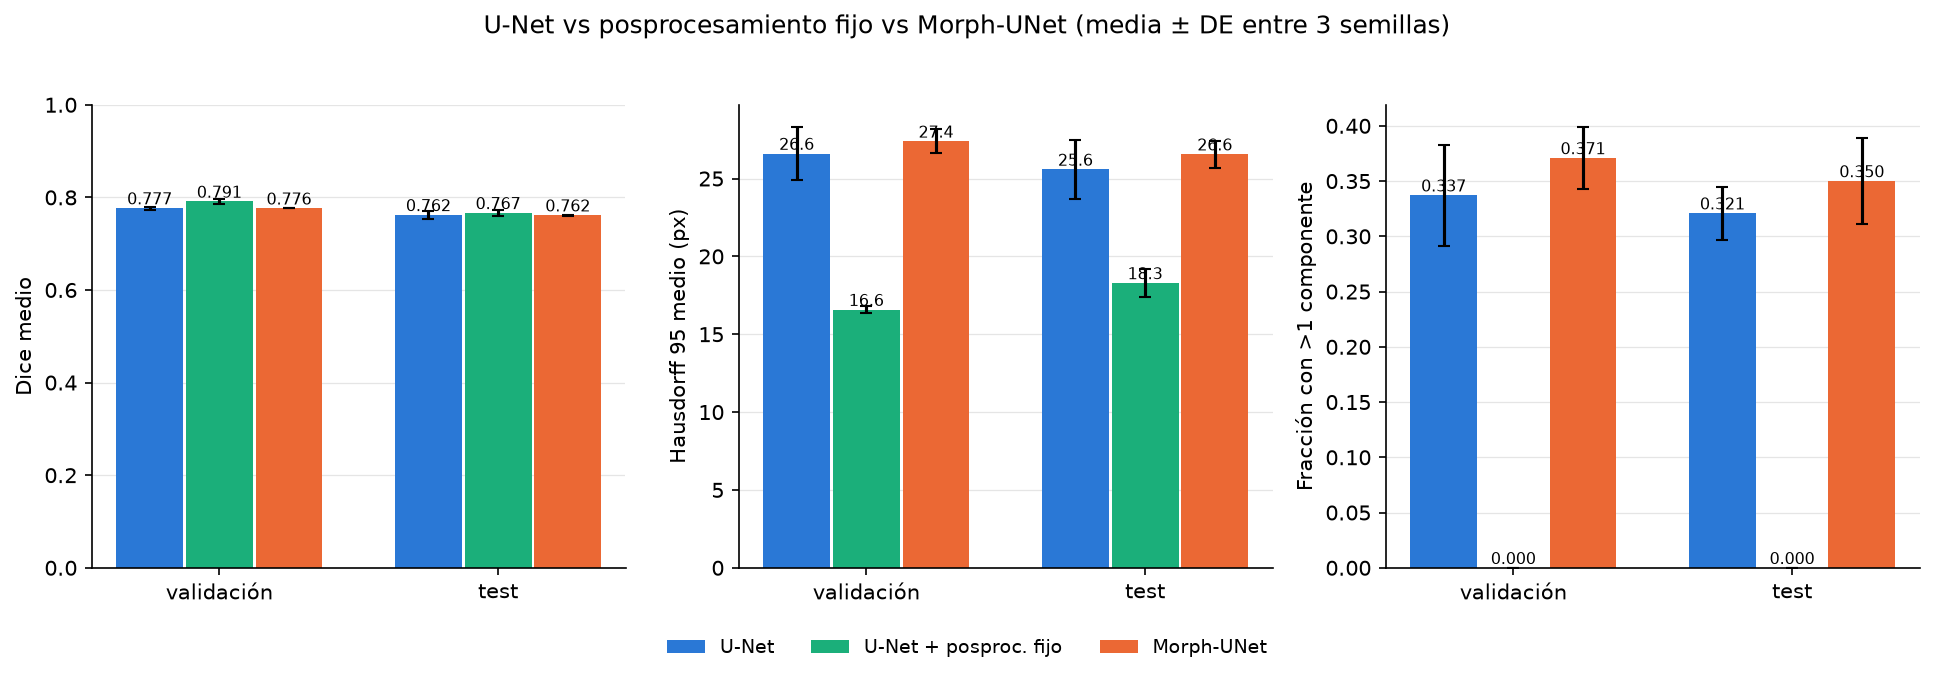
\includegraphics[width=0.95\linewidth]{morfologia_comparacion.png}
  \caption{U-Net, U-Net con posprocesamiento fijo y Morph-UNet (media $\pm$ DE de 3 semillas).}
  \label{fig:morfologia}
\end{figure}

\subsection{Otra familia de modelos: SegFormer-B0}
SegFormer-B0 es el mejor segmentador probado (Tabla~\ref{tab:principal}): en test, Dice $0.792 \pm 0.003$ frente a $0.762 \pm 0.009$ de la U-Net, es decir, $+0.030$ [IC 95\,\% por paciente $0.019$, $0.041$], Wilcoxon $p<10^{-4}$, con las 3 semillas por encima, y el HD95 medio baja 8.5 px. Frente a la U-Net con posprocesamiento la ventaja en test es $+0.026$ ($p=0.019$). La mejora proviene sobre todo de la sensibilidad (0.87 frente a 0.80) y de no dejar nunca una predicción vacía; a cambio, la precisión baja un poco. El posprocesamiento no aporta sobre SegFormer ($+0.001$): ya produce una sola componente en la mayoría de los casos.

\paragraph{Controles: arquitectura frente a preentrenamiento.} El codificador de SegFormer está preentrenado en ImageNet y la U-Net no, y además tiene el doble de parámetros, por lo que se entrenó SegFormer-B0 sin preentrenamiento. El Dice de validación escala así: U-Net $0.777$, SegFormer sin preentrenar $0.801$, preentrenado $0.810$. La diferencia atribuible a la arquitectura es $+0.024$ [IC 95\,\% $0.012$, $0.038$], $p=0.002$ (cerca del 74\,\% de la ventaja total; en test, $+0.020$ [$0.010$, $0.031$]); la atribuible al preentrenamiento es $+0.008$ [$-0.002$, $0.019$], $p=0.86$ (cerca del 26\,\%, no concluyente; en test $+0.010$ [$-0.001$, $0.020$]). El preentrenamiento sobre todo acelera la convergencia (mejor época 14--22 frente a 39--40). Un control del lr de la U-Net ($3\times10^{-4}$, solo semilla 42 y solo validación) dio 0.784 frente a 0.781, de modo que el lr no explica la diferencia.

\begin{figure}[H]
  \centering
  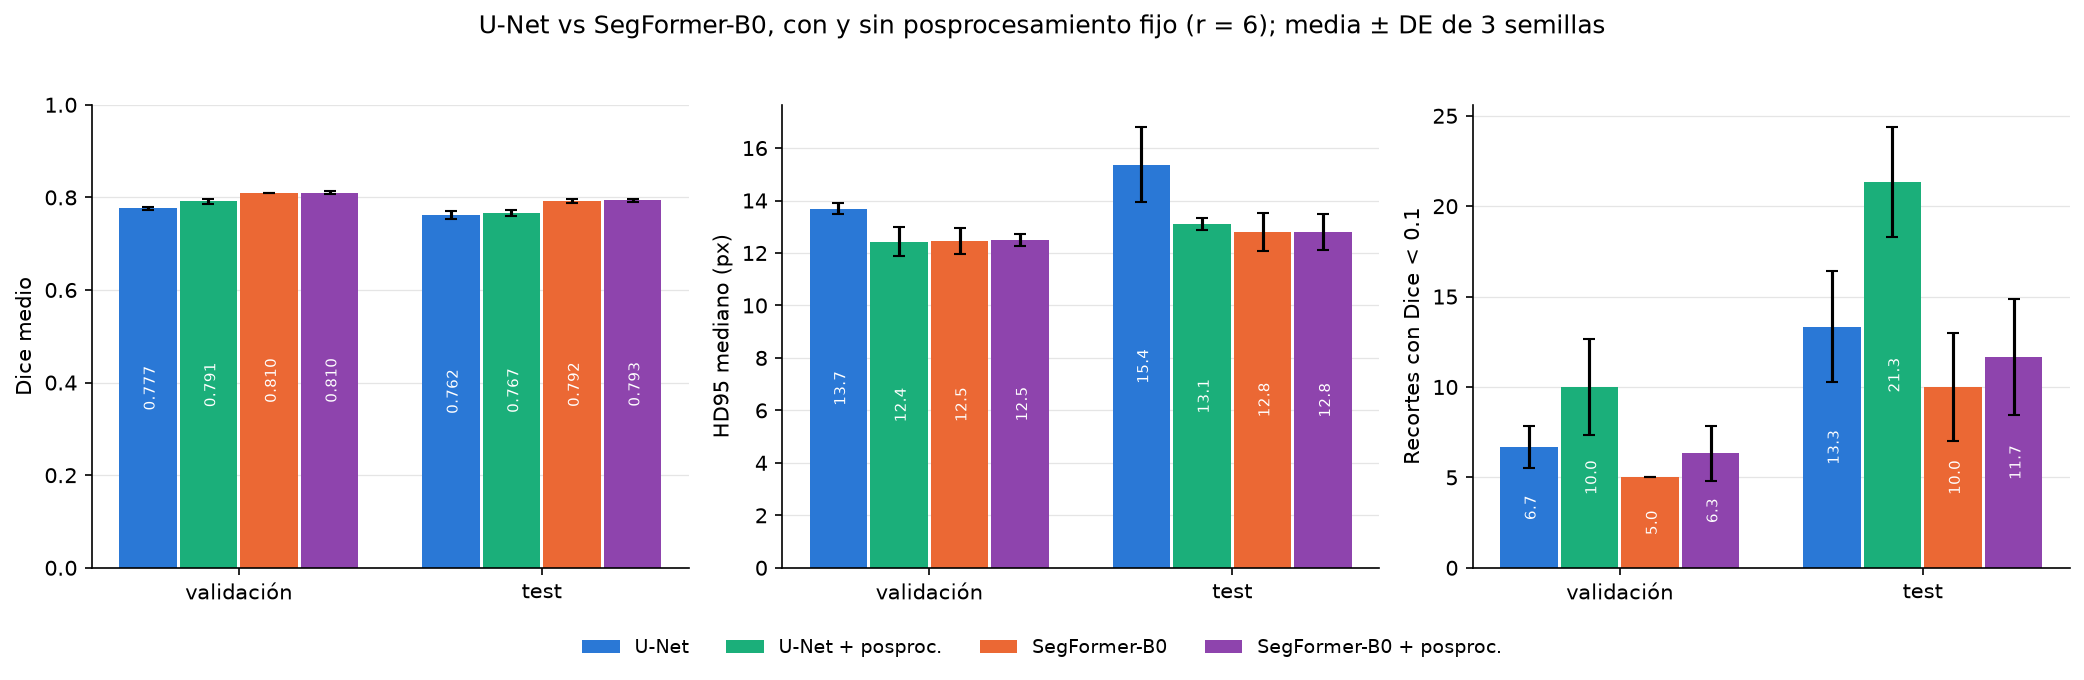
\includegraphics[width=0.95\linewidth]{segformer_comparacion.png}
  \caption{U-Net frente a SegFormer-B0, con y sin posprocesamiento fijo (media $\pm$ DE de 3 semillas).}
  \label{fig:segformer}
\end{figure}

\begin{figure}[H]
  \centering
  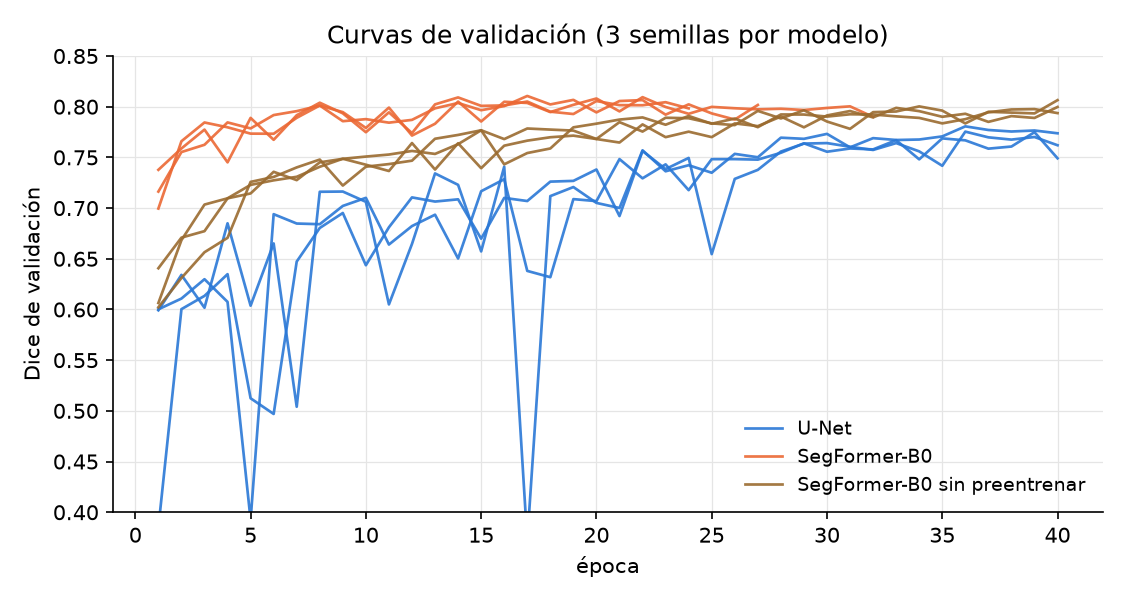
\includegraphics[width=0.95\linewidth]{segformer_controles_curvas.png}
  \caption{Dice de validación por época: U-Net, SegFormer-B0 preentrenado y sin preentrenar (3 semillas cada uno). Los modelos sin preentrenar llegan al tope de 40 épocas.}
  \label{fig:segformer-controles}
\end{figure}

\begin{figure}[H]
  \centering
  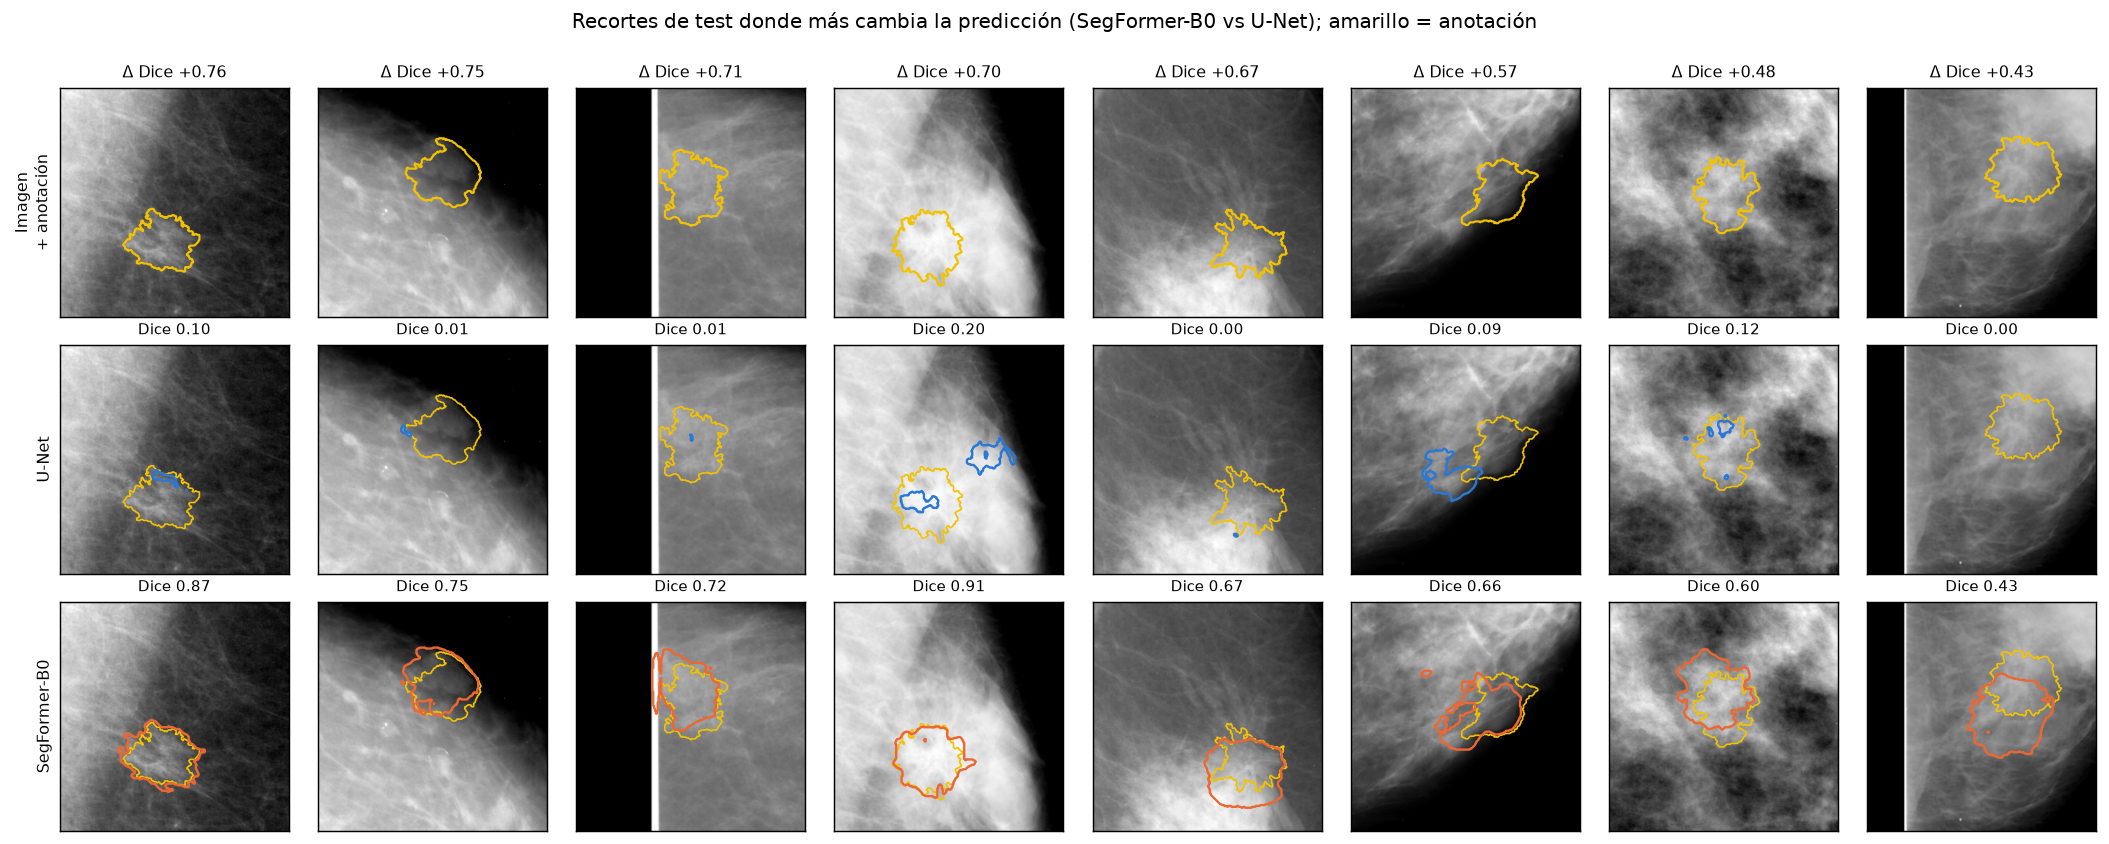
\includegraphics[width=0.95\linewidth]{segformer_ejemplos.png}
  \caption{Casos de test donde SegFormer-B0 y la U-Net más difieren: la U-Net marca un fragmento de la lesión y SegFormer la cubre entera.}
  \label{fig:segformer-ejemplos}
\end{figure}

\subsection{Dónde falla}\label{sec:fallos}
\paragraph{Por subgrupo.} La Tabla~\ref{tab:estrat} (test, Dice de la U-Net promediado por recorte entre semillas) muestra que lo que más pesa es la \emph{dificultad de la imagen}, no el tipo de lesión: las lesiones sutiles y las mamas densas bajan el Dice entre 0.15 y 0.25 y duplican el HD95 mediano (de 12 a 24 px), y ambas diferencias resisten la corrección de Holm. Entre las 4 formas básicas el Dice varía poco (0.78--0.82); la diferencia significativa la produce el grupo ``otras'' (distorsión arquitectural, ganglio, asimetrías; no son masas propiamente dichas). Margen, patología y vista no son significativos tras Holm. Los $p$ son optimistas, porque varios recortes son del mismo paciente y sutileza y densidad están correlacionadas.

\begin{table}[H]
\centering\small
\caption{Dice de la U-Net en test por subgrupo (3 semillas promediadas; Kruskal-Wallis, $p$ ajustado por Holm sobre 18 pruebas).}
\label{tab:estrat}
\begin{tabular}{p{2.6cm}p{8.4cm}p{3.2cm}}
\toprule
Variable & Grupos (Dice medio) & $p$ ($p_{\text{Holm}}$) \\
\midrule
Sutileza & 1: 0.58 ($n=14$) · 2: 0.62 · 3: 0.75 · 4: 0.78 · 5: 0.82 & $10^{-9}$ ($2\times10^{-8}$) \\
Densidad mamaria & 1: 0.85 · 2: 0.79 · 3: 0.71 · 4: 0.68 & $8\times10^{-7}$ ($10^{-5}$) \\
Forma & redonda 0.82 · ovalada 0.79 · lobulada 0.78 · irregular 0.78 · otras 0.61 & $4\times10^{-5}$ ($5\times10^{-4}$) \\
Margen & circunscrito 0.81 · microlobulado 0.82 · obscured 0.77 · mal definido 0.76 · espiculado 0.72 · mixto 0.72 & 0.014 (0.12, n.s.) \\
Patología & benigna 0.75 · maligna 0.79 & 0.30 (n.s.) \\
Vista & CC 0.77 · MLO 0.76 & 0.84 (n.s.) \\
\bottomrule
\end{tabular}
\end{table}

\begin{figure}[H]
  \centering
  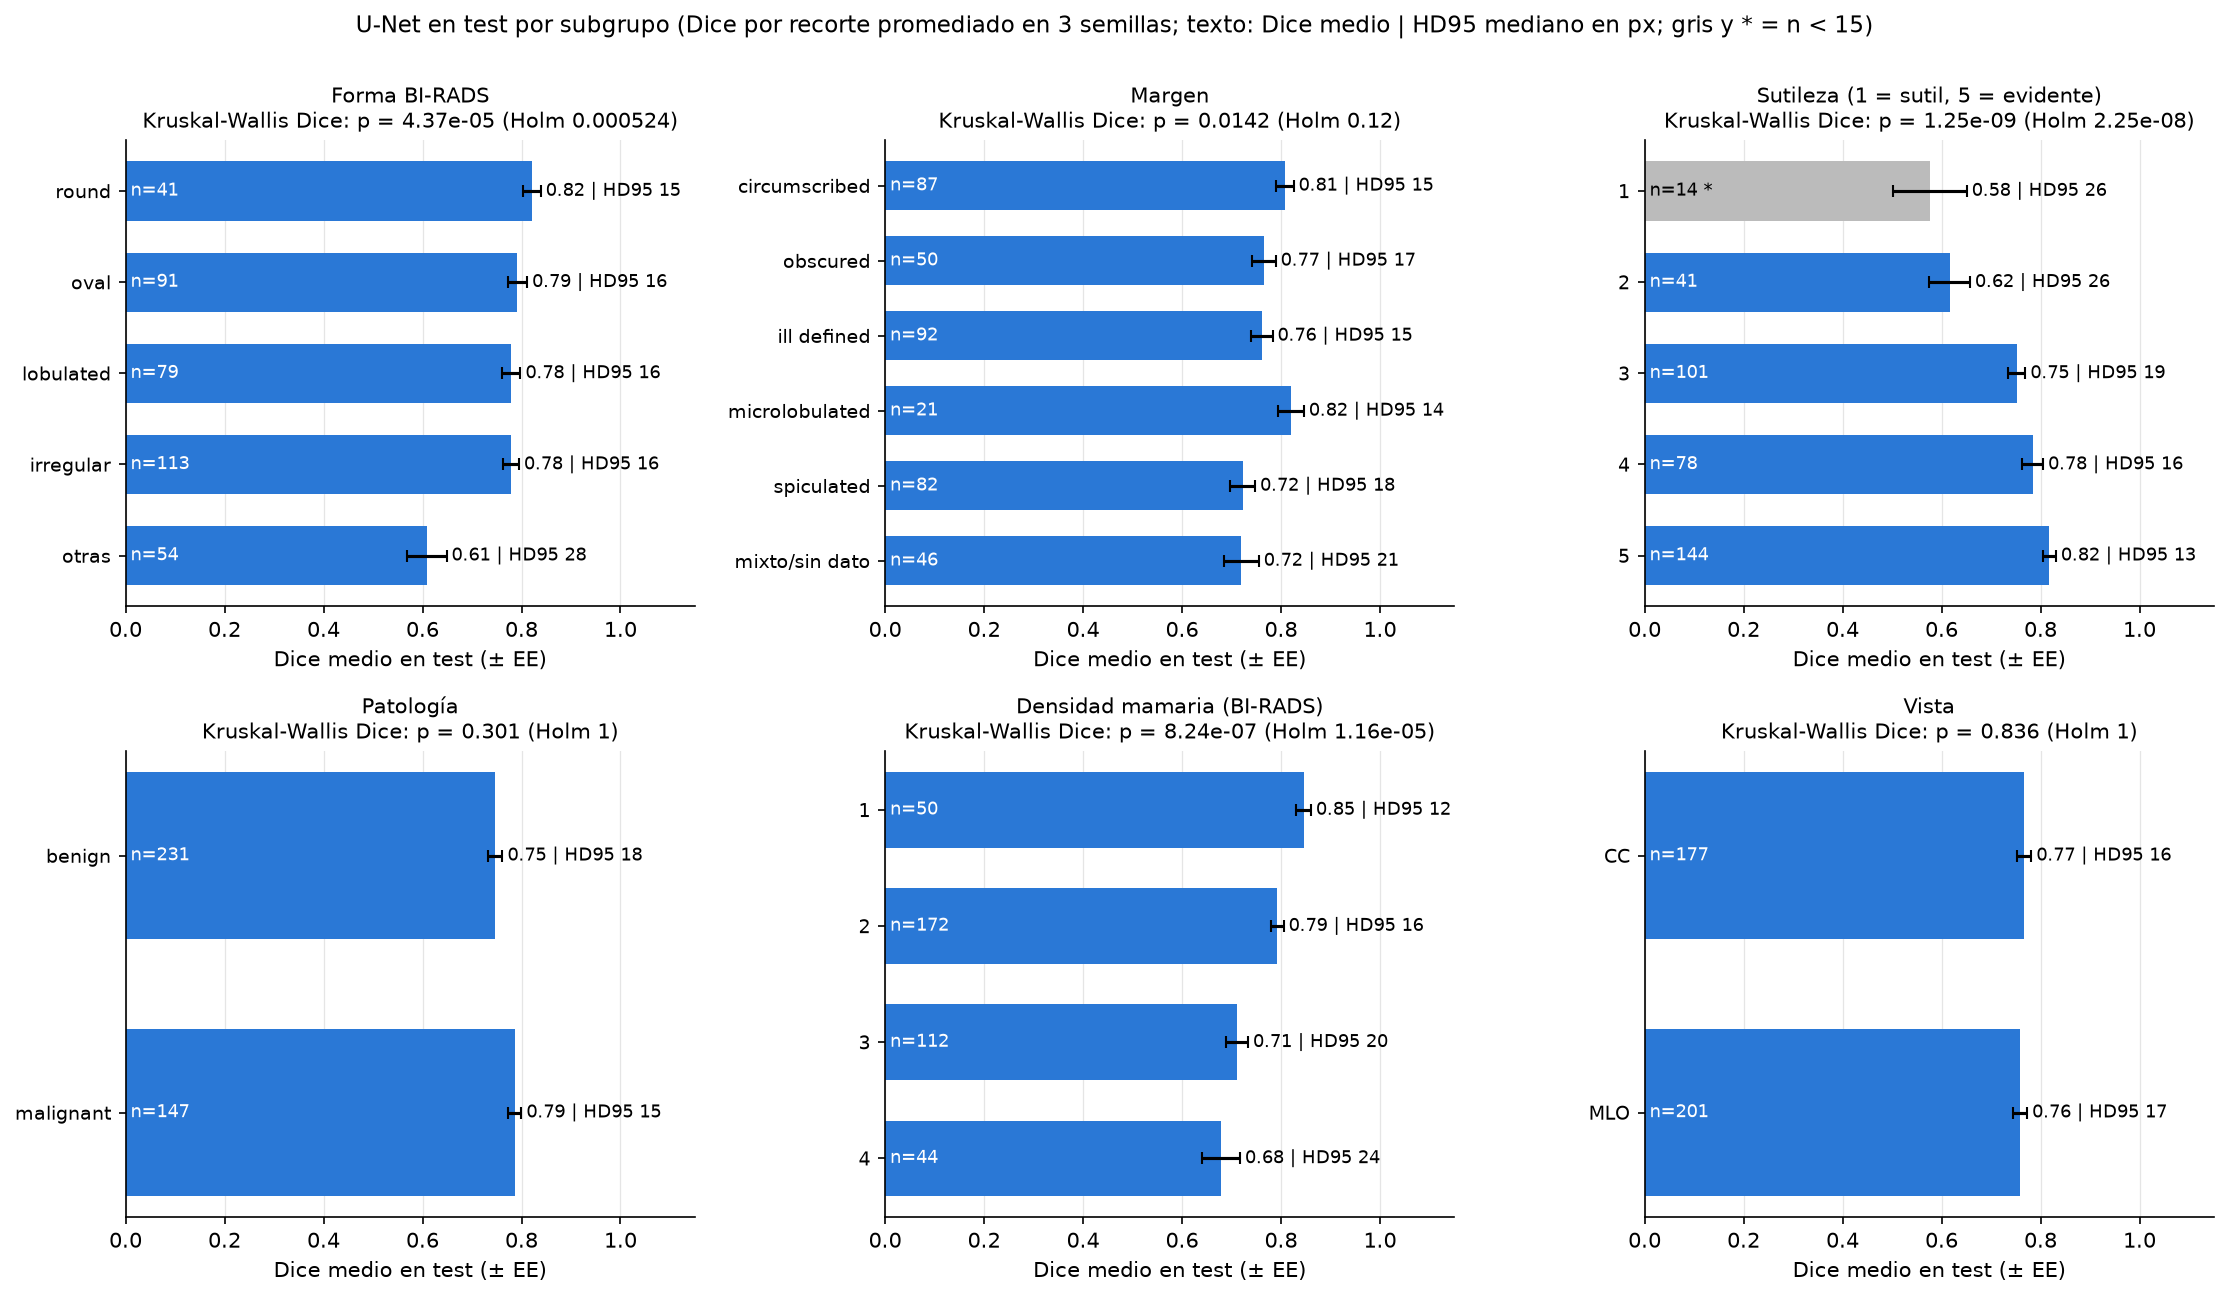
\includegraphics[width=0.95\linewidth]{estratificado_test.png}
  \caption{Dice en test por subgrupo.}
  \label{fig:estratificado}
\end{figure}

\paragraph{Modos de fallo.} Con la semilla 42, 16 de 378 recortes (4.2\,\%) tienen Dice $<0.1$ (las semillas 43 y 44 tienen 14 y 10): 2 predicciones vacías (una lesión cortada por el borde de la mamografía), 7 en otra zona sin solape y 7 de sub o sobresegmentación (en su mayoría también localizaciones en otra estructura que apenas toca la lesión). Es un problema de \emph{localización}, no de contorno. El desplazamiento los explica solo en parte: 9 de 16 caen en el tercil de mayor desplazamiento (mediana 0.19 frente a 0.15, $p=0.044$), pero también son lesiones más pequeñas ($p=0.0006$), más sutiles ($p=0.048$) y en mamas densas (12 de 16 con densidad 3--4).

\paragraph{¿Evita SegFormer ese modo de fallo?} La hipótesis era que la atención global le permitiría fallar menos al elegir otra estructura densa. \emph{No se confirma} (Tabla~\ref{tab:fallos2}): en test los fallos en ``otra zona'' pasan de 5.3 a 4.0 por semilla (McNemar $p=0.48$) y en validación incluso suben (de 1.0 a 4.3, $p=0.013$). SegFormer sí elimina las predicciones vacías. Los casos donde más gana son aquellos en que la U-Net marca solo un fragmento de la lesión (Figura~\ref{fig:segformer-ejemplos}): es una mejora en la detección de lesiones de bajo contraste, no en la elección de la estructura correcta.

\begin{table}[H]
\centering\small
\caption{Fallos (Dice $<0.1$) por modo, media por semilla; McNemar exacto emparejado.}
\label{tab:fallos2}
\begin{tabular}{lccccc}
\toprule
Modo & U-Net test & SegFormer test & $p$ test & U-Net val & SegFormer val \\
\midrule
Total & 13.3 & 10.0 & 0.14 & 6.7 & 5.0 \\
Predicción vacía & 2.3 & 0 & 0.016 & 3.0 & 0 \\
Otra zona sin solape & 5.3 & 4.0 & 0.48 & 1.0 & 4.3 ($p=0.013$) \\
Sub/sobresegmentación & 5.7 & 6.0 & 1.0 & 2.7 & 0.7 \\
\bottomrule
\end{tabular}
\end{table}

\begin{figure}[H]
  \centering
  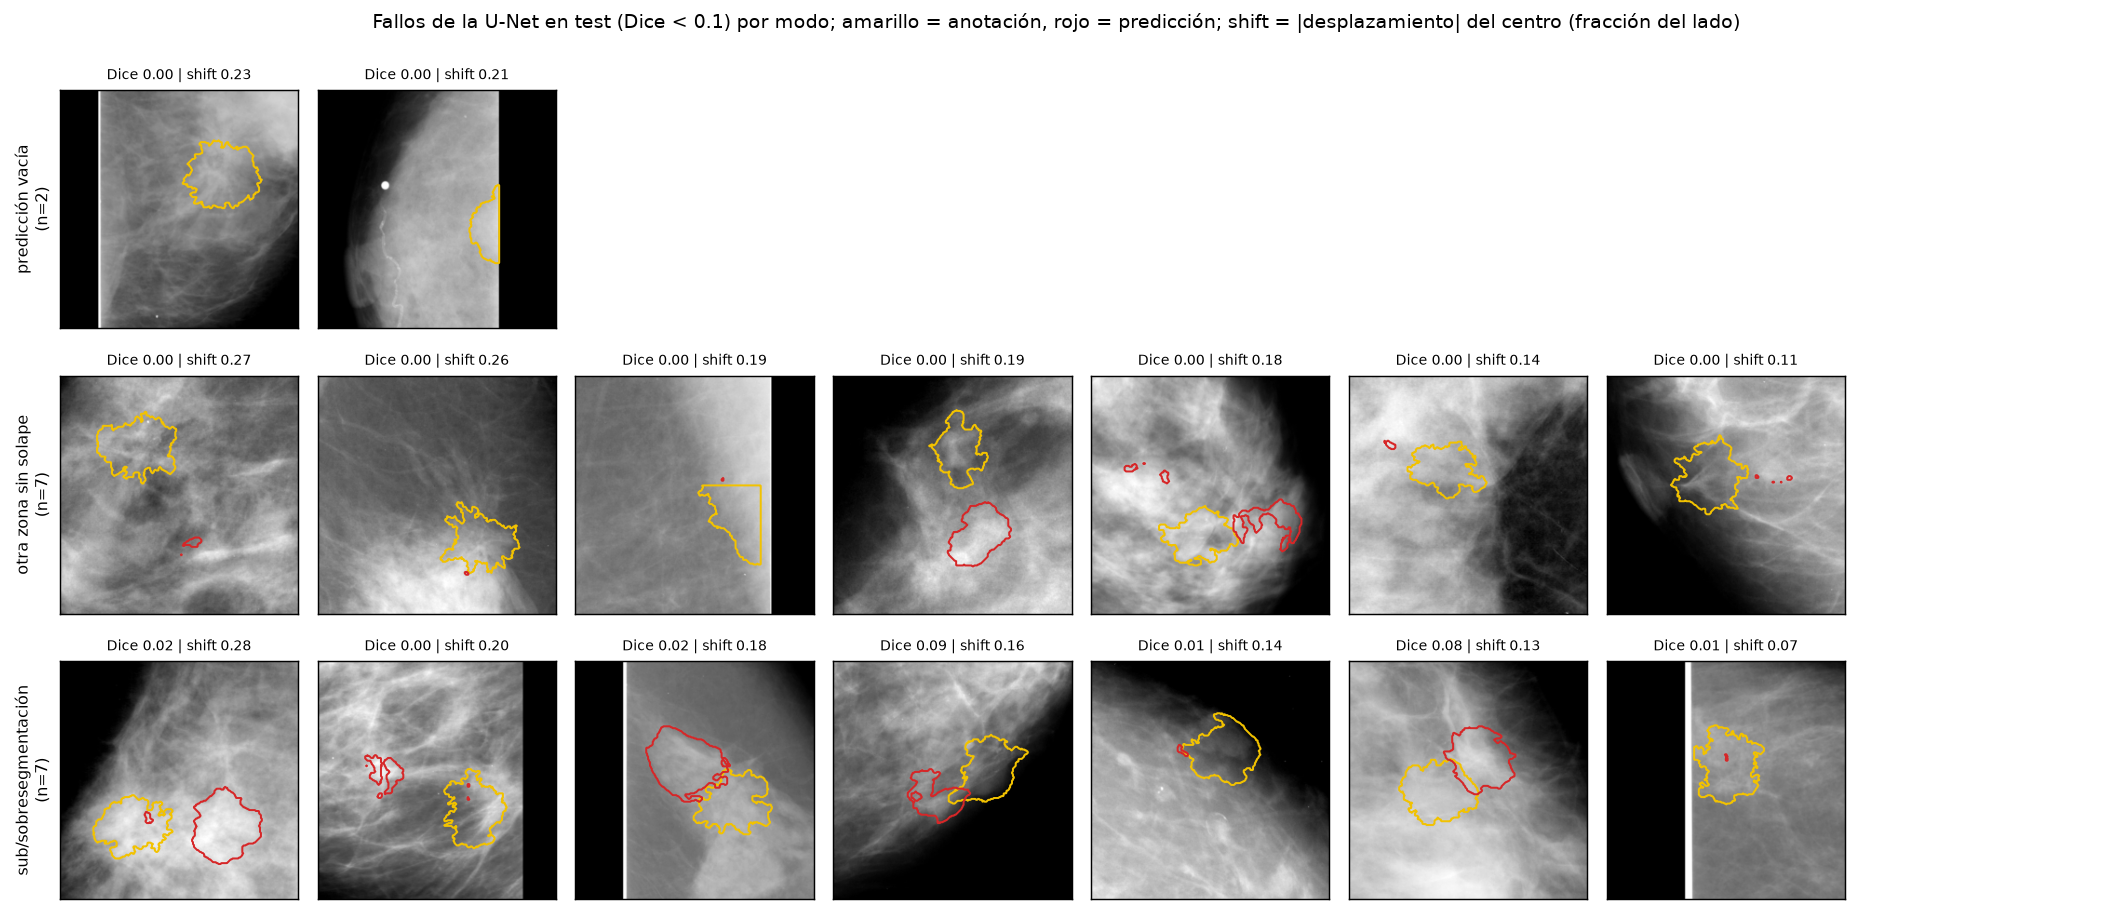
\includegraphics[width=0.95\linewidth]{fallos_por_modo.png}
  \caption{Recortes de test con Dice $<0.1$ por modo de fallo (U-Net, semilla 42).}
  \label{fig:fallos}
\end{figure}

\subsection{Forma y margen BI-RADS desde la máscara}\label{sec:forma}
\paragraph{La forma no se recupera.} El árbol de profundidad 3 queda al nivel del azar (0.25 en exactitud balanceada) incluso con las máscaras \emph{anotadas}: 0.220 con la máscara anotada y 0.249 con la de la U-Net (E1); con la mejor combinación elegida en validación (suavizado $\sigma=4$, árbol), 0.263 y 0.294, respectivamente, cuando predecir siempre la clase mayoritaria da 0.250 (Tabla~\ref{tab:ctrl}). Como el problema no está en la U-Net, se diseñaron controles. La etiqueta de forma del radiólogo \emph{sí} contiene información clínica (predice la patología con AUC 0.78), pero los descriptores geométricos de la máscara no (AUC $\approx 0.5$), ni siquiera para distinguir redonda de irregular (AUC 0.58 con regresión logística). Se descartó un error de procesamiento: cada recorte coincide con su fila del CSV y el interior de la máscara es más brillante que el exterior en el 98\,\% de los casos.

\begin{table}[H]
\centering\small
\caption{Controles de forma y margen en test (ajuste en entrenamiento, elección en validación, test una sola vez). El azar es AUC 0.5.}
\label{tab:ctrl}
\begin{tabular}{lcc}
\toprule
Tarea & $n$ & AUC \\
\midrule
Patología $\leftarrow$ solo descriptores & 324 & 0.490 \\
Forma regular vs.\ irregular $\leftarrow$ descriptores & 324 & 0.493 \\
Redonda vs.\ irregular $\leftarrow$ descriptores (regresión logística) & 154 & 0.581 \\
Patología $\leftarrow$ tamaño de la lesión & 378 & 0.608 \\
Patología $\leftarrow$ \textbf{etiqueta de forma} del radiólogo & 324 & \textbf{0.780} \\
Patología $\leftarrow$ descriptores + etiqueta de forma & 324 & 0.756 \\
Margen no circunscrito $\leftarrow$ descriptores (M1) & -- & 0.646 \\
Margen espiculado $\leftarrow$ descriptores (M2) & -- & 0.500 \\
Patología $\leftarrow$ \textbf{etiqueta de margen} del radiólogo & -- & \textbf{0.782} \\
Patología $\leftarrow$ descriptores + etiqueta de margen & -- & 0.807 \\
\bottomrule
\end{tabular}
\end{table}

\paragraph{El margen tampoco.} La geometría recupera apenas el margen circunscrito frente al no circunscrito (AUC en test 0.646; 0.587 en validación) y nada la espiculación (0.500), mientras que la etiqueta de margen sí predice la patología (AUC 0.78). Sumar los descriptores a la etiqueta de margen no ayuda en validación (0.860 frente a 0.868); la diferencia en test (0.807 frente a 0.782) no es evidencia de mejora. Las máscaras de CBIS-DDSM no dibujan las espículas.

\paragraph{Las máscaras de las redes sesgan hacia ``lobulada''.} Con el árbol ajustado sobre máscaras anotadas, las máscaras predichas se clasifican como ``lobulada'' en el 63--82\,\% de los casos (U-Net 75\,\%, U-Net con posprocesamiento 82\,\%, Morph-UNet 73\,\%, SegFormer-B0 70\,\%), frente al 24\,\% de las etiquetas reales: los contornos predichos son más suaves y redondeados que los anotados. Ninguna máscara, ni de la red ni anotada, recupera la forma (exactitud balanceada 0.22--0.31, cerca del azar de 0.25, y los valores más altos en test no se repiten en validación).

\begin{figure}[H]
  \centering
  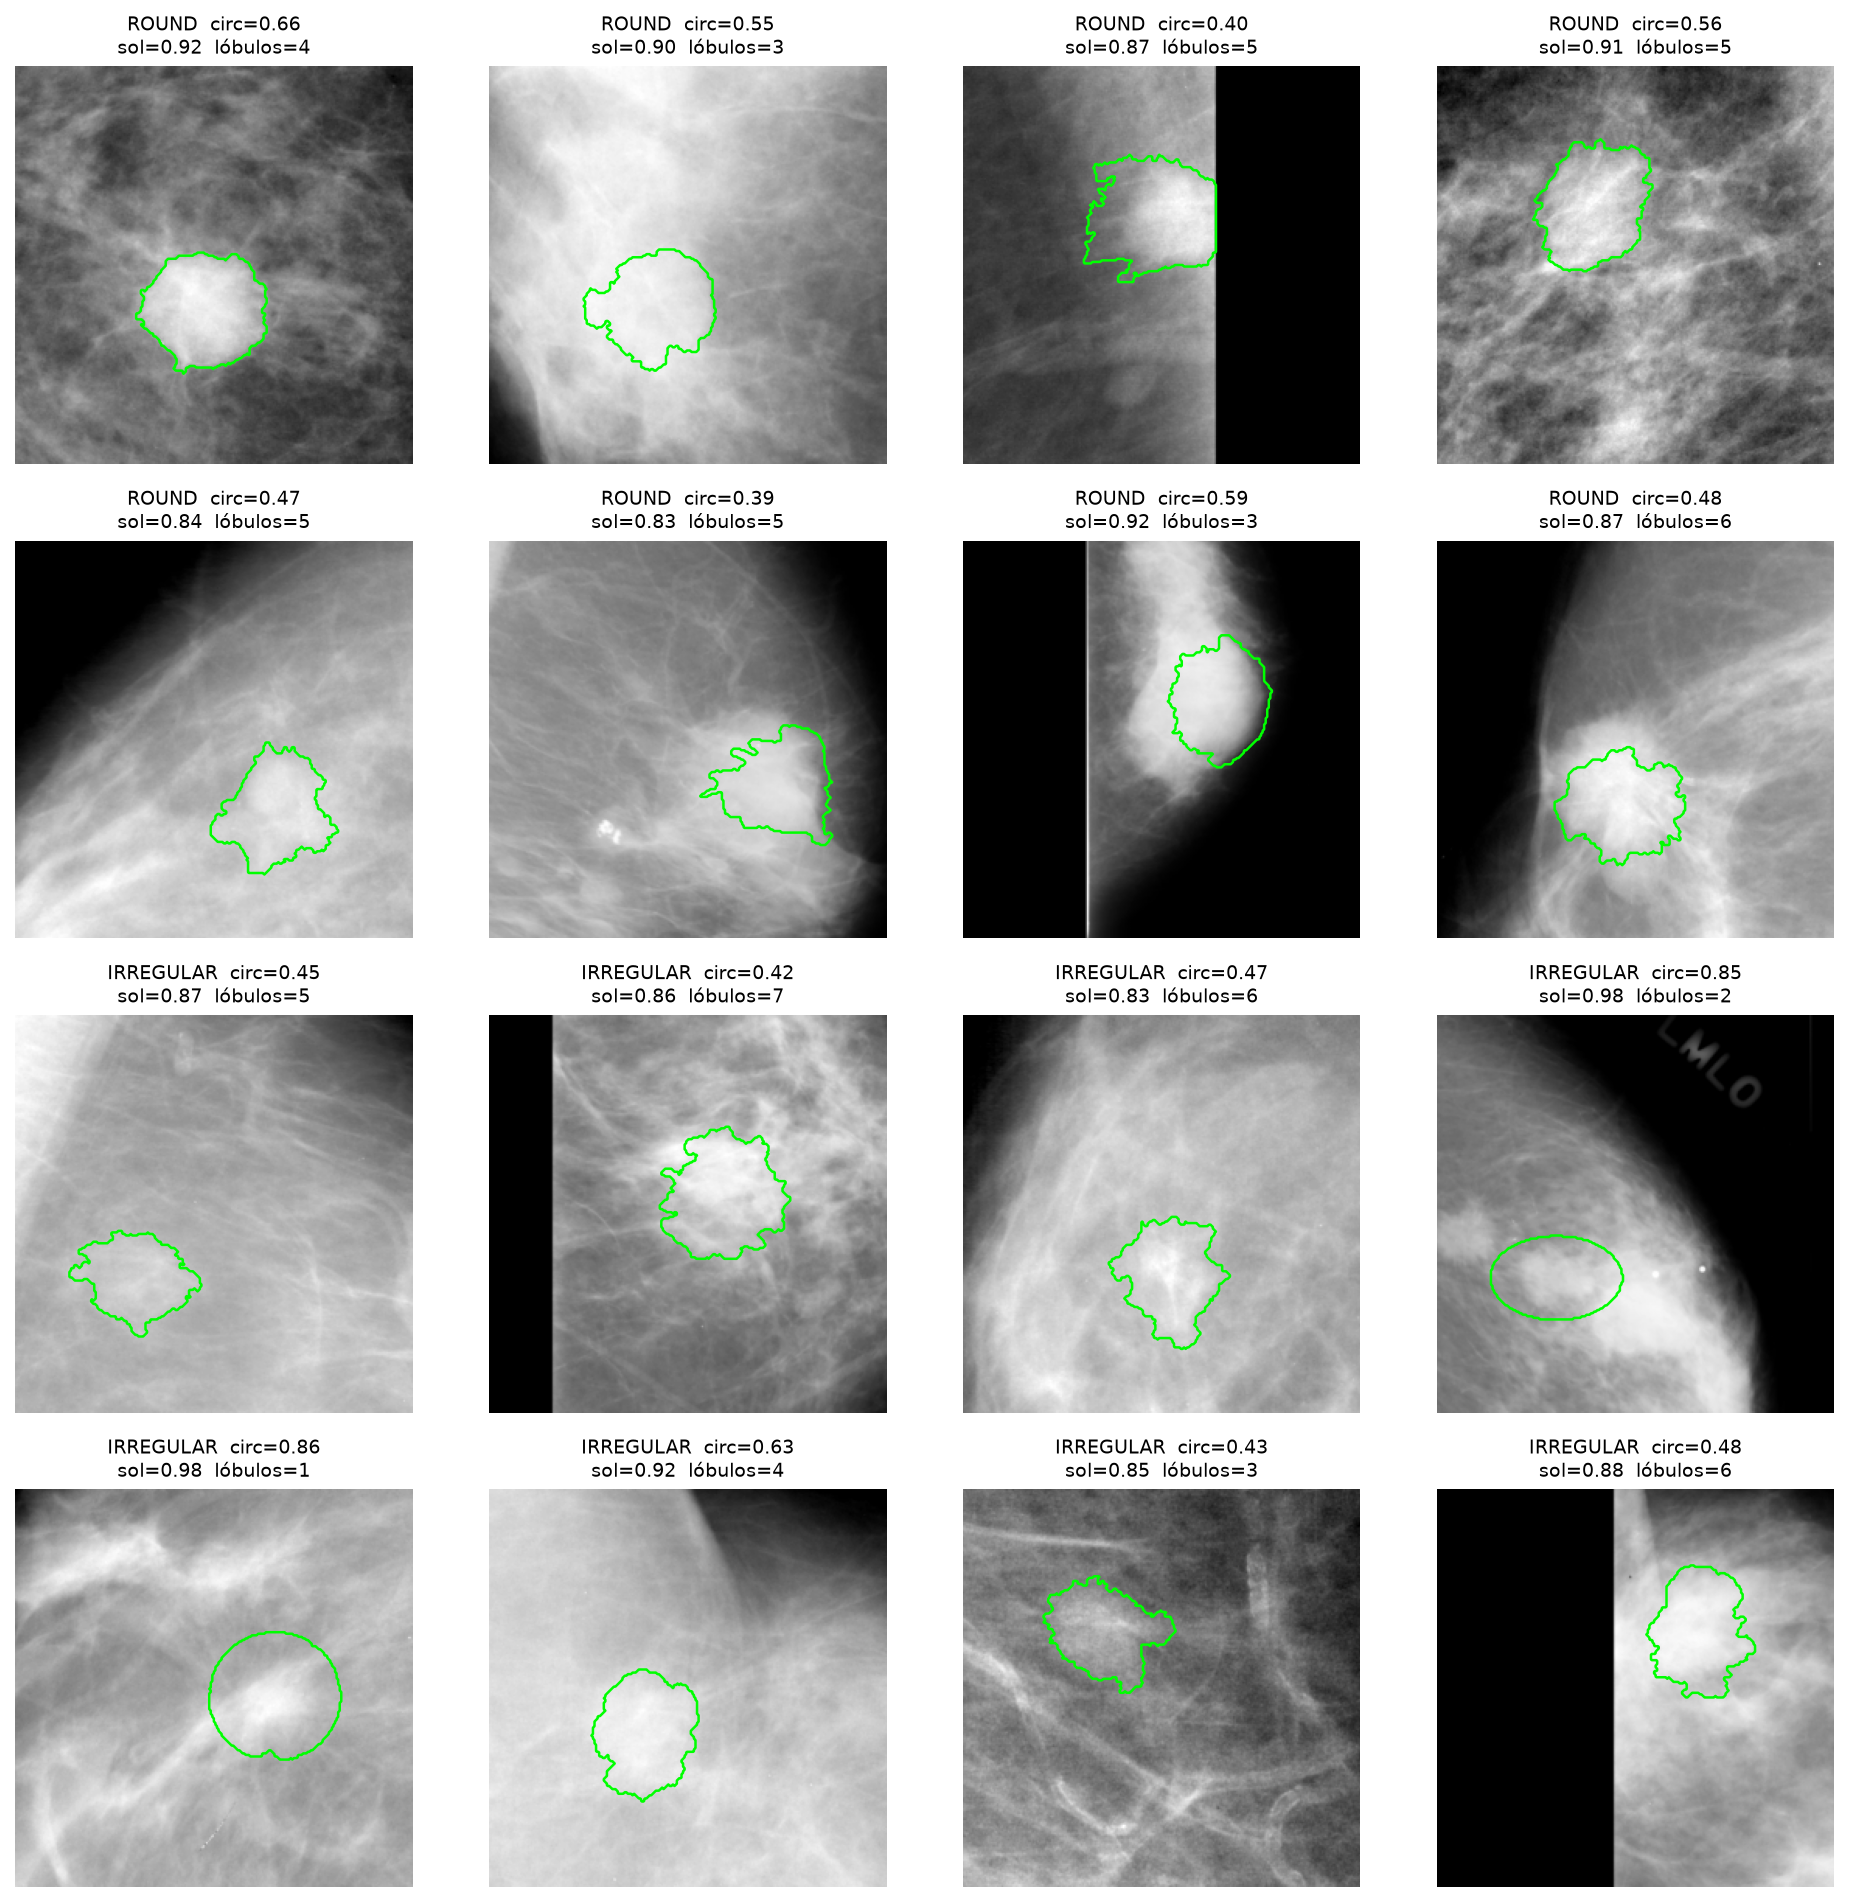
\includegraphics[width=\linewidth]{diagnostico_mascaras.png}
  \caption{Ocho máscaras anotadas ``redondas'' y ocho ``irregulares'' con circularidad, solidez y número de lóbulos: visualmente no se distinguen.}
  \label{fig:mascaras}
\end{figure}

\begin{figure}[H]
  \centering
  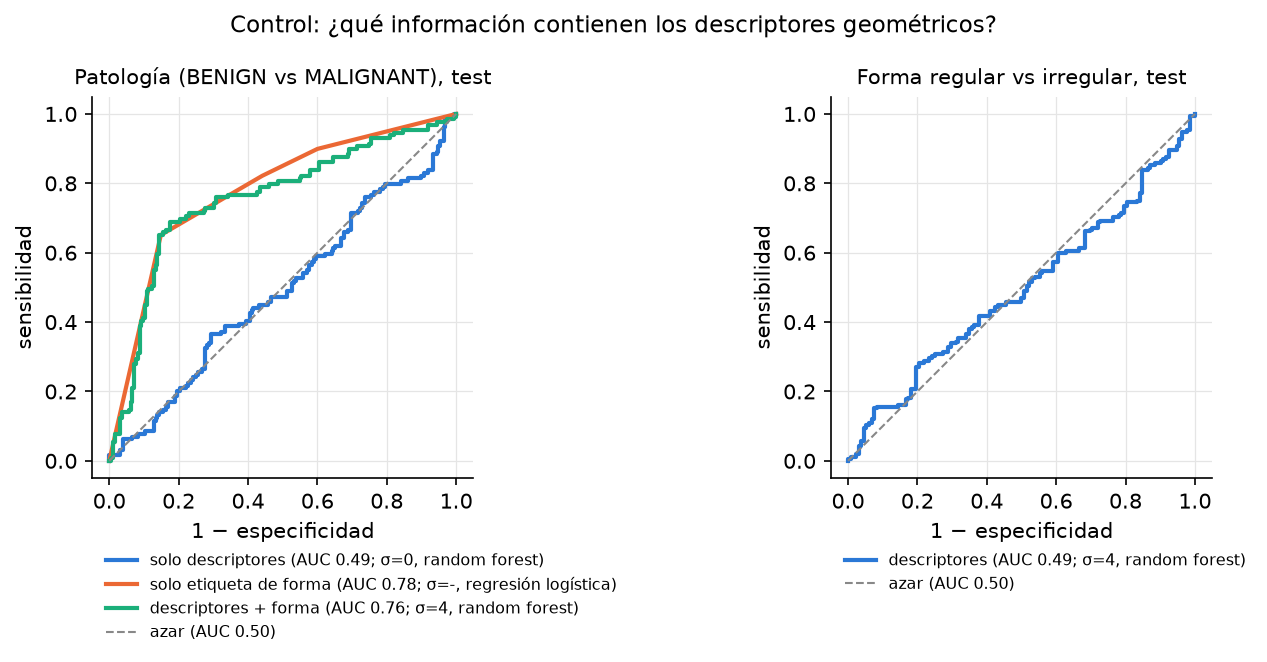
\includegraphics[width=0.95\linewidth]{control_forma_roc.png}
  \caption{Controles de forma: curvas ROC en test.}
  \label{fig:control-forma}
\end{figure}

\begin{figure}[H]
  \centering
  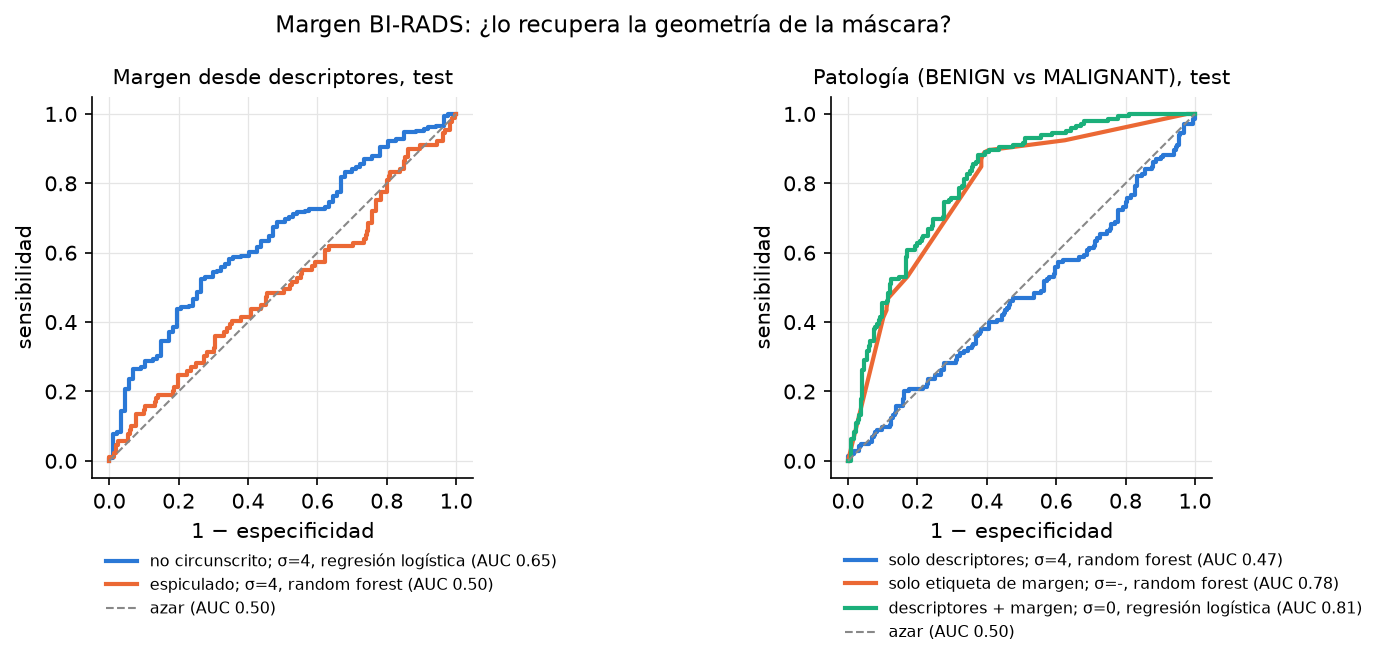
\includegraphics[width=0.95\linewidth]{margen_roc.png}
  \caption{Margen desde los descriptores y patología desde el margen.}
  \label{fig:margen}
\end{figure}

%==================================================================
\section{Discusión}
\paragraph{La métrica depende del diseño del recorte.} El resultado más instructivo del proyecto no es un número de Dice sino el atajo de posición: con recortes centrados en la lesión, un círculo fijo supera a la U-Net. El Dice de este problema solo es interpretable junto con un control de posición y con el desplazamiento aleatorio del ROI, y por eso las cifras aquí no son comparables con las de la literatura que segmenta mamografías completas u otros protocolos \citep{abdelhafiz2020,baccouche2021connected}.

\paragraph{Qué mejora el modelo y qué no.} La morfología, tanto aprendible dentro de la red como fija, no resuelve el problema de fondo, que es de localización: la red, igual que un transformer con atención global, a veces segmenta otra estructura densa con apariencia de masa. Lo que sí aporta la morfología fija es una limpieza del contorno (HD95), que en la práctica es la selección de la componente mayor y no la apertura o el cierre. SegFormer mejora el Dice sobre todo por una mayor sensibilidad, y la mayor parte de esa ventaja persiste sin preentrenamiento, de modo que no se explica solo por el preentrenamiento de ImageNet ni, según la evidencia disponible, por una menor confusión con otras estructuras densas.

\paragraph{El Dice sigue la dificultad de la imagen.} El rendimiento baja con la sutileza y con la densidad mamaria, no con la patología, la vista ni la forma básica de la lesión. Las lesiones pequeñas, sutiles y en mamas densas concentran los fallos graves.

\paragraph{El límite de la forma está en las máscaras, no en la red.} La etiqueta del radiólogo predice la patología (AUC $\approx0.78$ para forma y para margen), pero los mismos descriptores calculados sobre la máscara anotada no (AUC $\approx 0.5$): las máscaras ROI de CBIS-DDSM son contornos toscos, sin espículas, e independientes de la forma anotada. Una explicación plausible, \emph{no verificada} aquí, es que los contornos fueron refinados automáticamente a partir de la anotación original \citep{lee2017cbisddsm}, por lo que no representan el borde que el radiólogo usó para juzgar la forma. Segmentar mejor no corrige esto: con las máscaras de cuatro modelos distintos el resultado es el mismo. Como trabajo futuro, una base con máscaras de mejor calidad o mamografía digital moderna, como VinDr-Mammo \citep{nguyen2023vindr}, sujeta al acceso por PhysioNet, permitiría reabrir la pregunta.

%==================================================================
\section{Limitaciones}
\begin{itemize}
\item CBIS-DDSM proviene de película digitalizada de los años 90, no de mamografía digital moderna; la generalización a equipos actuales no está garantizada.
\item El recorte se construye a partir de la caja de la lesión, con desplazamiento aleatorio, de modo que la posición aproximada es conocida. No es un sistema de detección; el control ``prior centrado'' mide cuánto se explica solo por la posición.
\item Las máscaras ROI no representan con fidelidad el contorno; esto impide derivar forma y margen en este conjunto con independencia de la calidad de la segmentación. Las etiquetas de forma y margen tienen variabilidad entre lectores y no hay segunda lectura.
\item Solo 3 semillas; las ablaciones usan una sola. Diferencias de alrededor de 0.01 no se distinguen del ruido. Los resultados en GPU varían ligeramente entre ejecuciones (cuDNN no es determinista).
\item Los $p$ del análisis estratificado son optimistas: varios recortes son del mismo paciente y las variables están correlacionadas.
\item \textbf{Controles de SegFormer.} (a) Los modelos sin preentrenar y la U-Net con lr $3\times10^{-4}$ llegaron al tope de 40 épocas con la mejor época en la 39--40: la comparación vale ``con un presupuesto de 40 épocas'' y no dice dónde convergerían. (b) La época 1 de cada SegFormer fue más lenta (42--48 s) por el calentamiento de CUDA. (c) El control de lr de la U-Net es de una sola semilla y solo en validación. (d) SegFormer tiene el doble de parámetros que la U-Net, y su lr solo se ajustó con 2 valores; el de la U-Net viene de la entrega parcial.
\item La Morph-UNet se comparó con 3 semillas y 40 épocas; la semilla 43 alcanzó su mejor época en la última. La inicialización de $p$ ($\pm5$) casi no cambió, y no se exploraron otras inicializaciones ni ubicaciones además de las dos probadas.
\item El análisis de sensibilidad del radio es posterior y descriptivo; la decisión $r=6$ se tomó en validación y se mantiene.
\end{itemize}

%==================================================================
\section{Conclusiones}
\begin{enumerate}
\item Una U-Net pequeña (1.94 M de parámetros) segmenta masas en recortes ROI de CBIS-DDSM con Dice $0.762 \pm 0.009$ en el test oficial, más del doble que el método clásico y el control de posición, y el resultado es estable entre semillas y particiones.
\item Sin desplazamiento aleatorio del ROI, un círculo fijo supera a la U-Net: el diseño del recorte condiciona la métrica.
\item La morfología aprendible en la red no mejora; la morfología fija mejora el contorno (HD95 de 25.6 a 18.3 px), casi por completo gracias a quedarse con la componente conexa mayor.
\item SegFormer-B0 es el mejor modelo (Dice test $0.792 \pm 0.003$, $+0.030$ sobre la U-Net). La ventaja se debe sobre todo a la arquitectura y no solo al preentrenamiento, y no proviene de evitar otras estructuras densas.
\item El rendimiento depende de la dificultad de la imagen (sutileza, densidad) y no del tipo de lesión; los fallos graves son de localización.
\item La forma y el margen BI-RADS no se recuperan desde las máscaras de CBIS-DDSM, ni siquiera desde las anotadas, aunque sus etiquetas sí predicen la patología: el límite está en las máscaras.
\end{enumerate}

%==================================================================
\appendix
\section{Reproducibilidad y materiales}\label{sec:repro}
\begin{itemize}
\item \textbf{Repositorio:} \url{https://github.com/Any64/mamo-seg} (privado, compartido con el equipo docente). Contiene \texttt{src/}, \texttt{scripts/}, \texttt{configs/}, \texttt{notebooks/}, \texttt{tests/}, \texttt{results/} (tablas y figuras) y este informe en \texttt{report/}. No incluye datos ni pesos.
\item \textbf{Ejecución principal:} \texttt{python scripts/run\_experiment.py --config configs/main.yaml}. Los experimentos E1--E13 y sus comandos están en el README.
\item \textbf{Pruebas:} \texttt{python -m pytest -q tests} (47 pruebas con dataset sintético).
\item \textbf{Video de la presentación:} \url{PENDIENTE}
\end{itemize}

\bibliographystyle{plainnat}
\bibliography{refs}
\end{document}
